\subsection{Advection Equation}\label{sec:advection}
\subsubsection{Problem Formulation}
We first consider the one-dimensional linear advection equation, with discontinuous residual $f$.
The problem has a simple analytical solution, serving as a sanity check for whether our implementation of the method has any merit.
The problem is defined by \eqref{eq:advection} below.
\begin{equation}
\begin{cases}
    u_t + \alpha \cdot u_x= 0 &\text{for } (x,t)\in [-1, 1] \times (0, 1] \\ 
    u(x, 0) = u_0(x)= f &\text{for } x \in [-1, 1],
\end{cases}
\label{eq:advection}
\end{equation}
where $\alpha = 0.5$, and the initial condition $f$ is defined by
\begin{equation*}
    f(x) =
    \begin{cases}
        1 &\text{if } x \in [-0.2, 0.2] \\
        0 &\text{else}.
    \end{cases}
\end{equation*}
By the method of characteristics, the analytical solution is
\begin{equation}
    u(x,t) = u_0(x-\alpha t) =
    \begin{cases}
        1 &\text{if } x - \alpha t \in  [-0.2, 0.2], \\
        0 &\text{else}.
    \end{cases}
\end{equation}

Thus, the problem defines a wave travelling rightwards without diffusion with a speed $\alpha$.
The analytical solution also predicts two discontinuities.
For our XPINN formulation, we decompose the domain according to the predicted discontinuities as in \autoref{fig:decomp_advection}.

\begin{figure}[h]
    \centering
    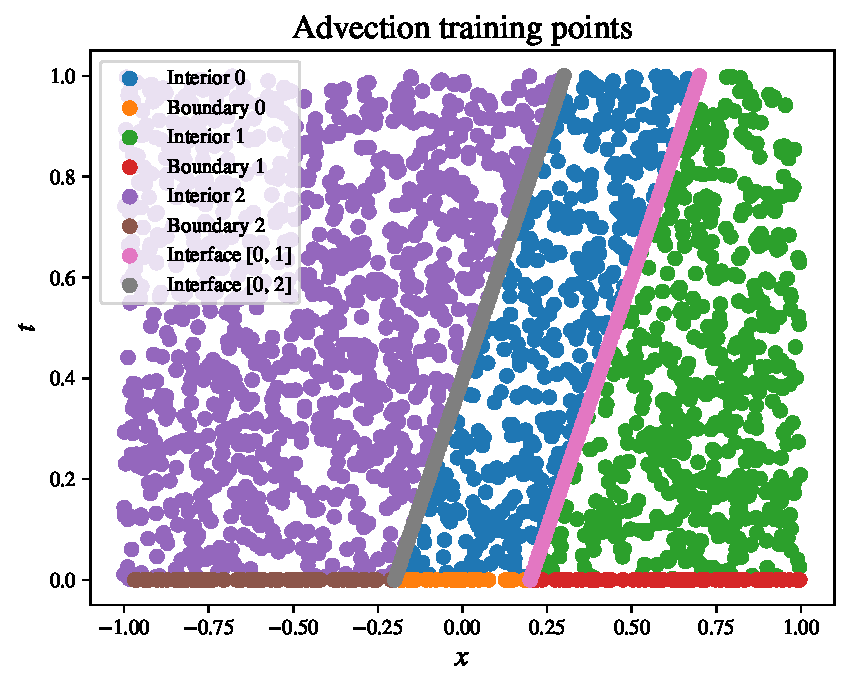
\includegraphics[width=0.8\linewidth]{Project1XPINNs/figures/advection/advection_train.pdf}
    \label{subfig:single}
    \caption{Training points for the advection equation with the domain decomposed into three subdomains.}
    \label{fig:decomp_advection}
\end{figure}

In order to verify that our method is not simply learning the decomposition itself, we also verify that the wave is able to travel across the interfaces by setting $\alpha = -1$ while keeping the same decomposition.
Finally we compare our XPINN model with a single PINN training on the entire domain without any subdomains. 

Our network is composed of $6$ hidden layers, each with $20$ nodes, using $\tanh$ as our hidden activation function and no activation for the output layer. The learning rate is set to $10^{-4}$, with \textsc{Adam} as the optimizer.
We utilize $2000$ points for the interior, and $200$ evenly spread around the boundary and interfaces. 

\subsubsection{Results}
We run the models for 10 000 epochs each.
The resulting predictions are seen in \autoref{fig:advection_xpinn_pred}, closely fitting the true solution.
The absolute errors against the true solution can be seen in \autoref{fig:advection_xpinn_error}, where most of the error is found along the interfaces.
This is unsurprising, given the discontinuities along the boundaries.


\begin{figure}[h]
    \centering
    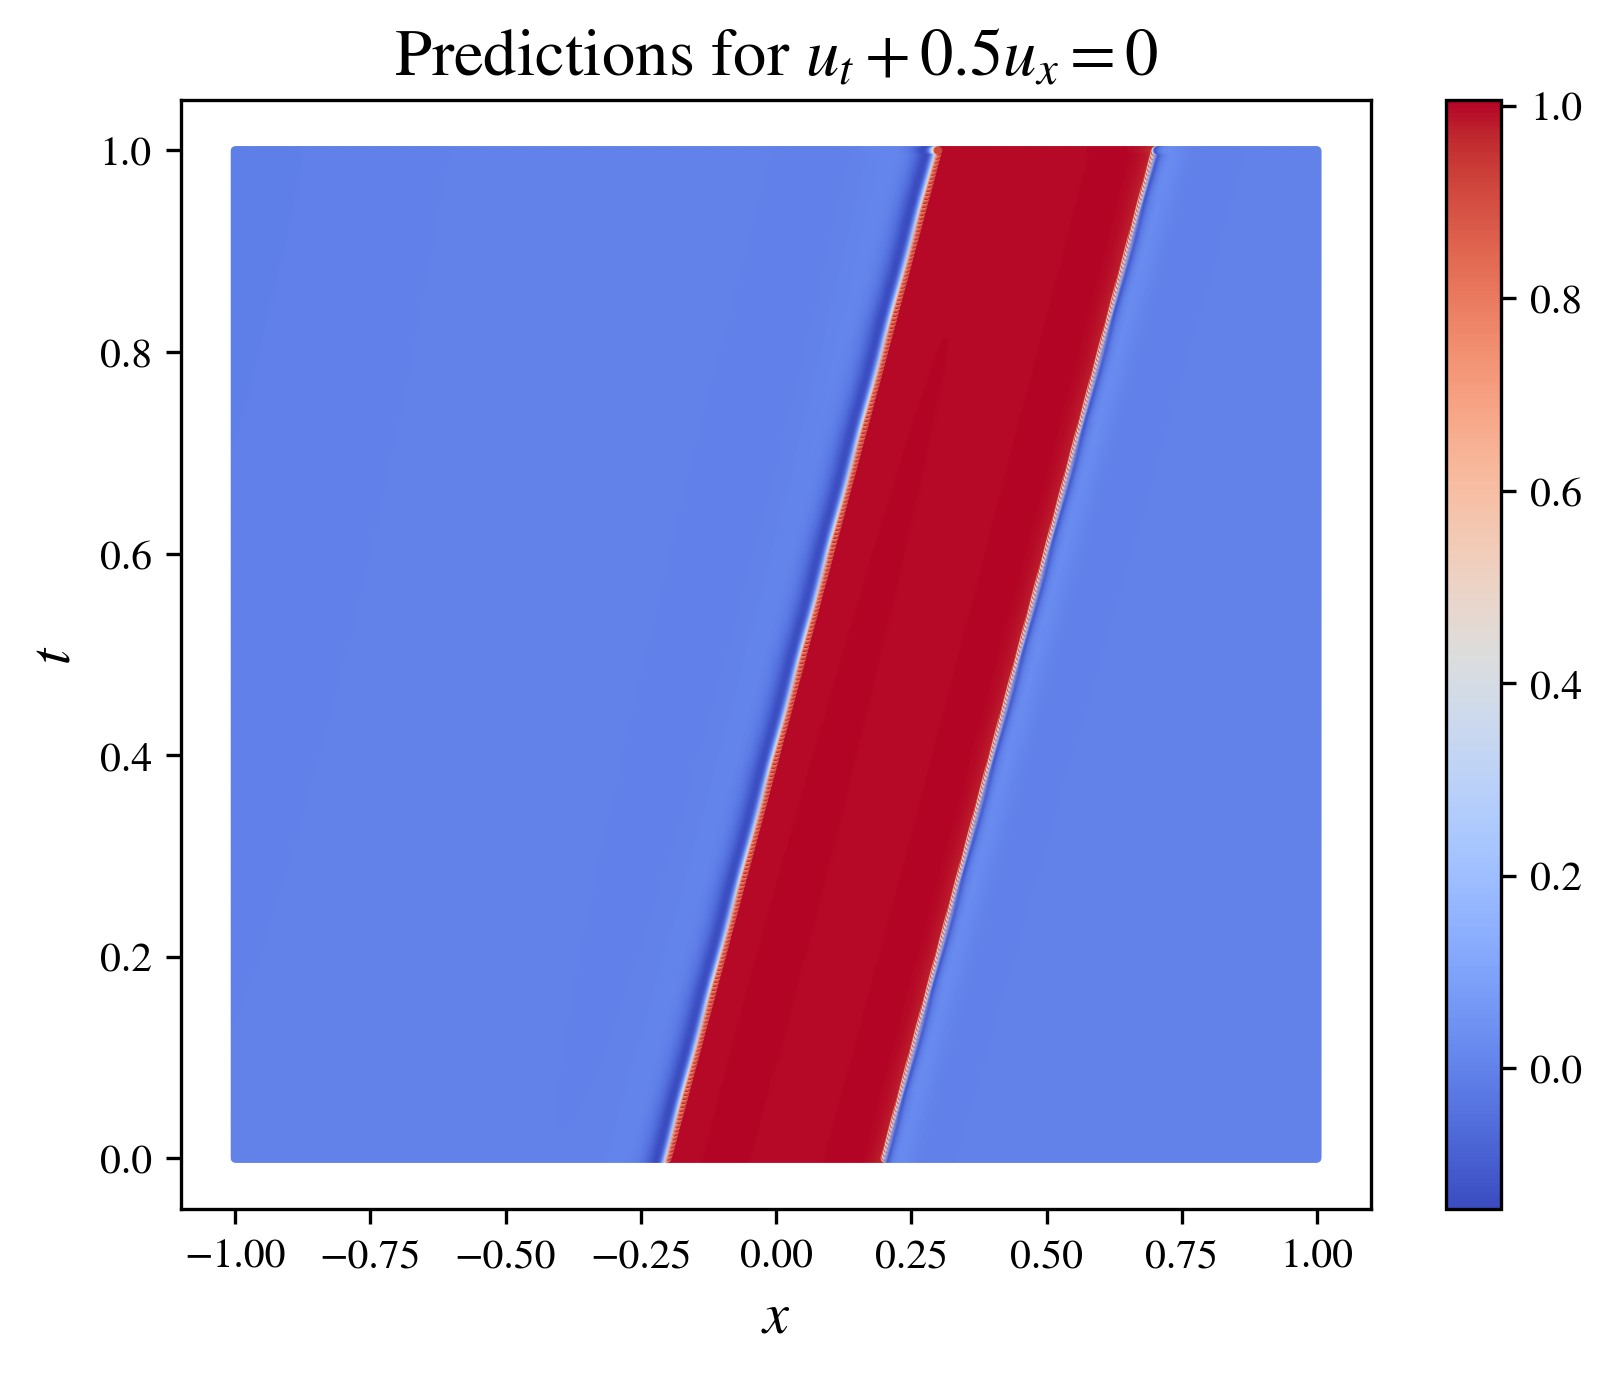
\includegraphics[width=0.7\linewidth]{Project1XPINNs/figures/advection/xpinn_predictions.png}
    \caption{Predictions for the advection equation with XPINN, $\alpha = 0.5$.}
    \label{fig:advection_xpinn_pred}
\end{figure}

\begin{figure}[h]
    \centering
    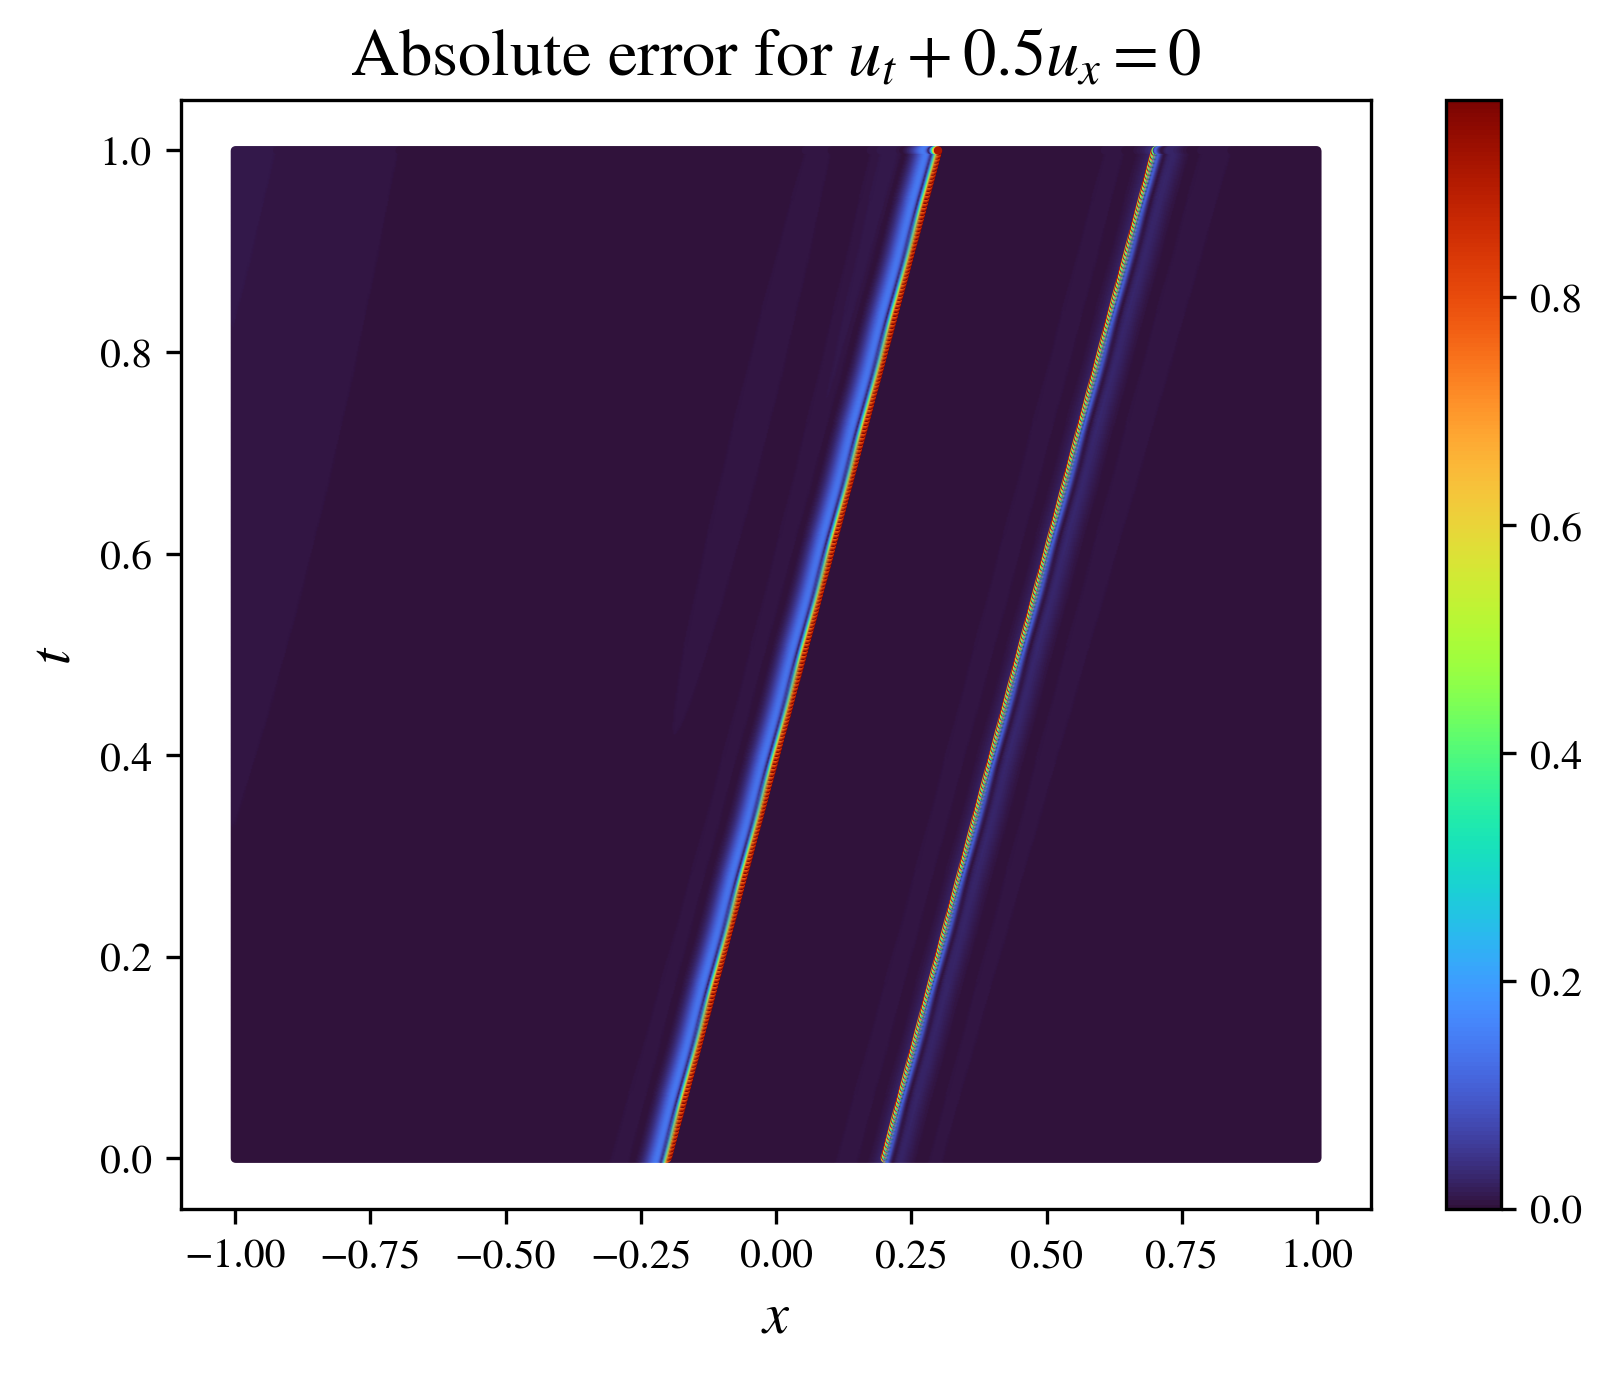
\includegraphics[width=0.7\linewidth]{Project1XPINNs/figures/advection/xpinn_error.png}
    \caption{Error against true solution, XPINN with $\alpha=0.5$.}
    \label{fig:advection_xpinn_error}
\end{figure}

The loss per epoch is shown in \autoref{fig:loss_per_advection}.
It is interesting to note how the different sub-PINNs adjust in accordance with each other, wherein the reduction in the loss of one sub-PINN often leads to an increase in the others, while the total loss is reduced.
Do note that the model seems to still be improving after 10 000 epochs, and that the learning rate needs further tuning.
We chose to not optimize this problem fully, as we were more interested in learning more about the behaviour of XPINNs, and seeing if our implementation had any merit.

\begin{figure}[h]
    \centering
    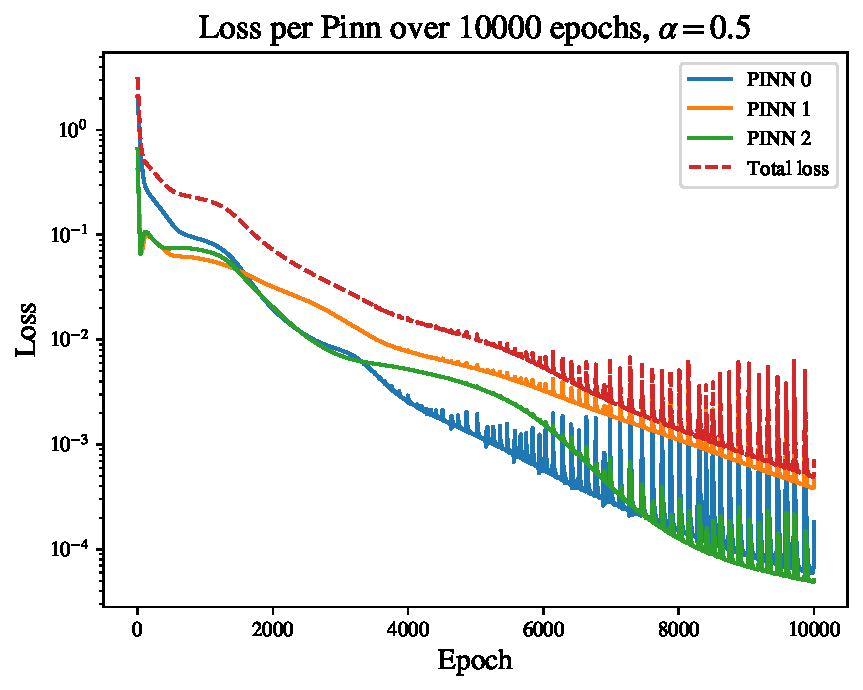
\includegraphics[width=0.8\linewidth]{Project1XPINNs/figures/advection/advection_losses.pdf}
    \caption{Loss per epoch for advection XPINN, with $\alpha=0.5$.}
    \label{fig:loss_per_advection}
\end{figure}

Comparing against how a single PINN on the entire domain performs, we see better and more stable results from running the same number of epochs.
The predicted values are shown in \autoref{fig:single_ad_pred}, with the errors in \autoref{fig:single_ad_error}.
XPINNs then probably do not have a lot of merit for such a simple problem, especially given the simplicity of deriving the analytical solution.

\begin{figure}[h]
    \centering
    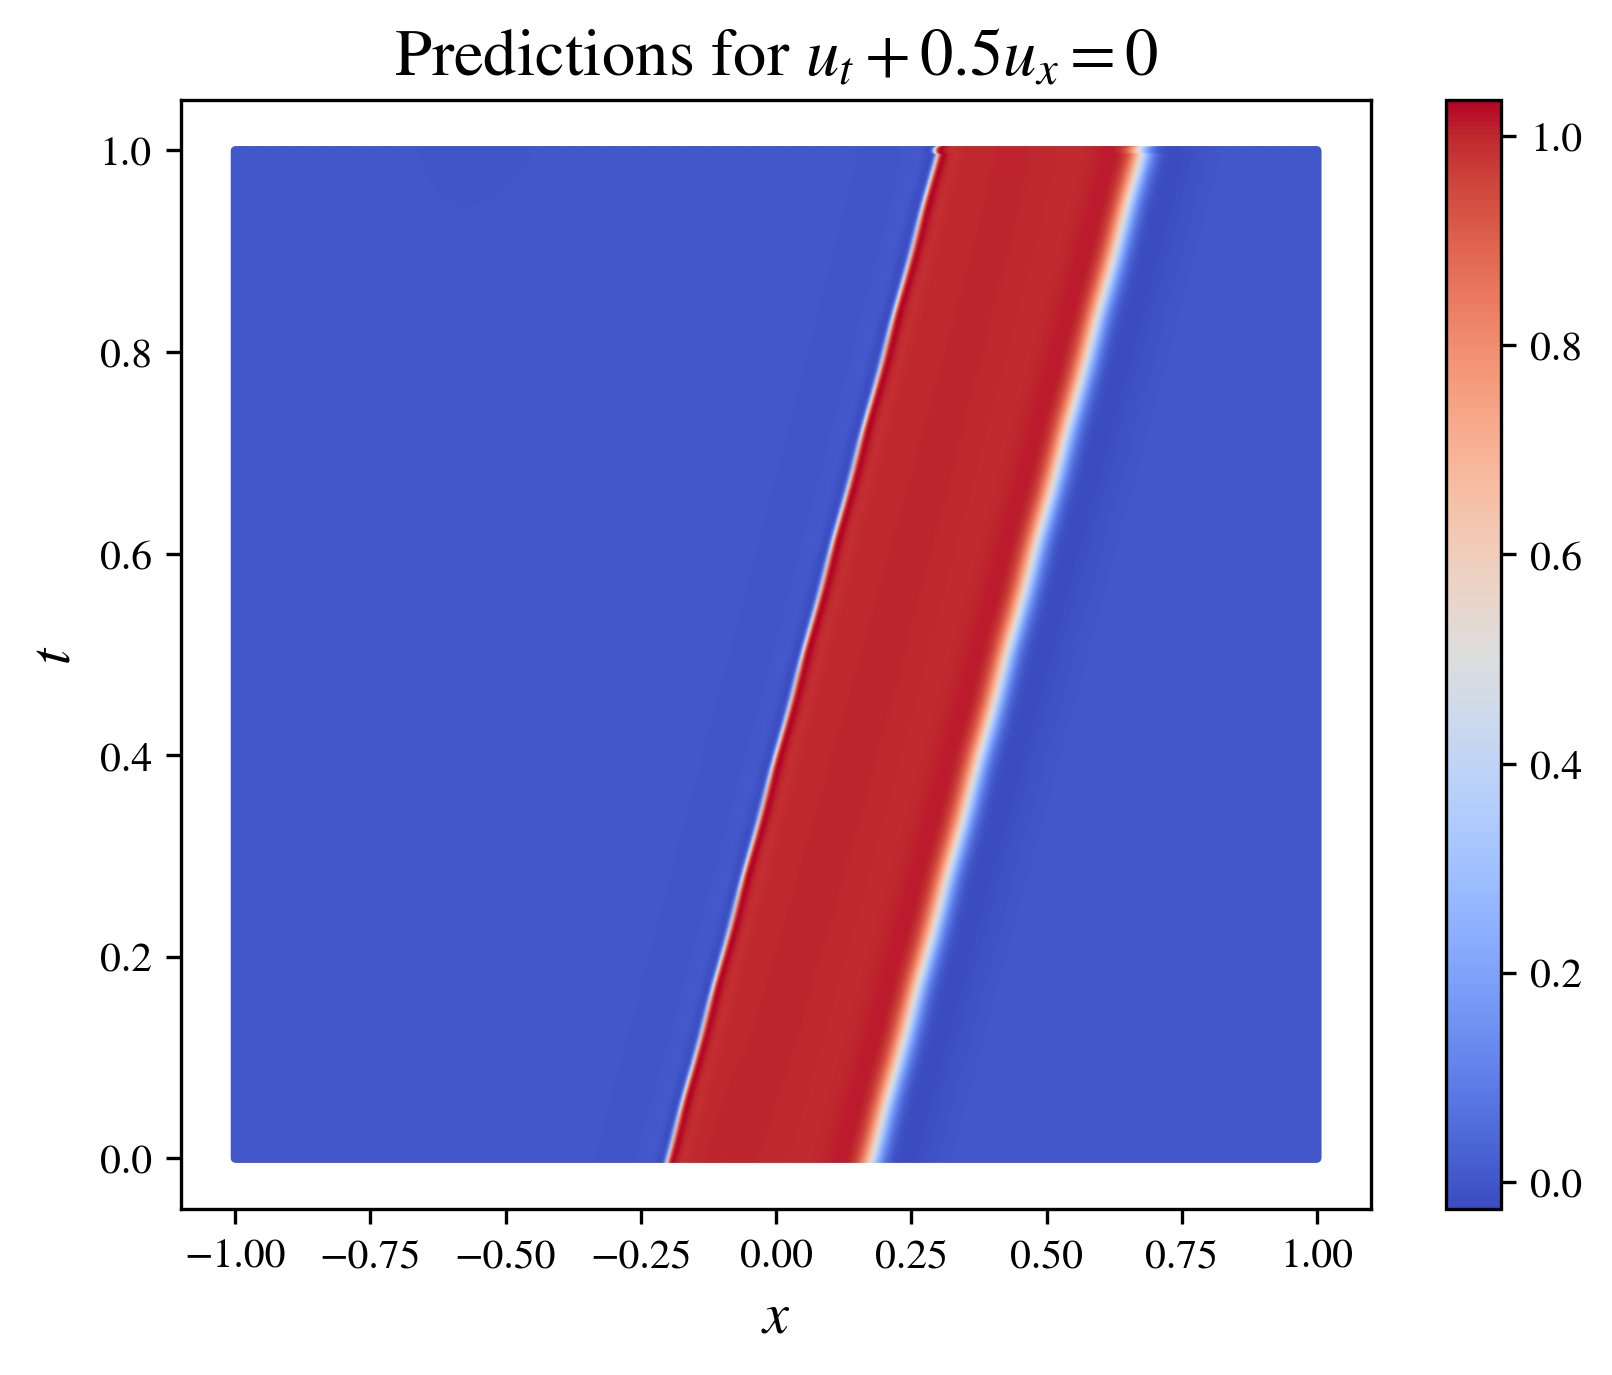
\includegraphics[width=0.8\linewidth]{Project1XPINNs/figures/advection/single_advection_predictions.png}
    \caption{Predicted values for the advection equation, with a single PINN.}
    \label{fig:single_ad_pred}
\end{figure}

\begin{figure}[h]
    \centering
    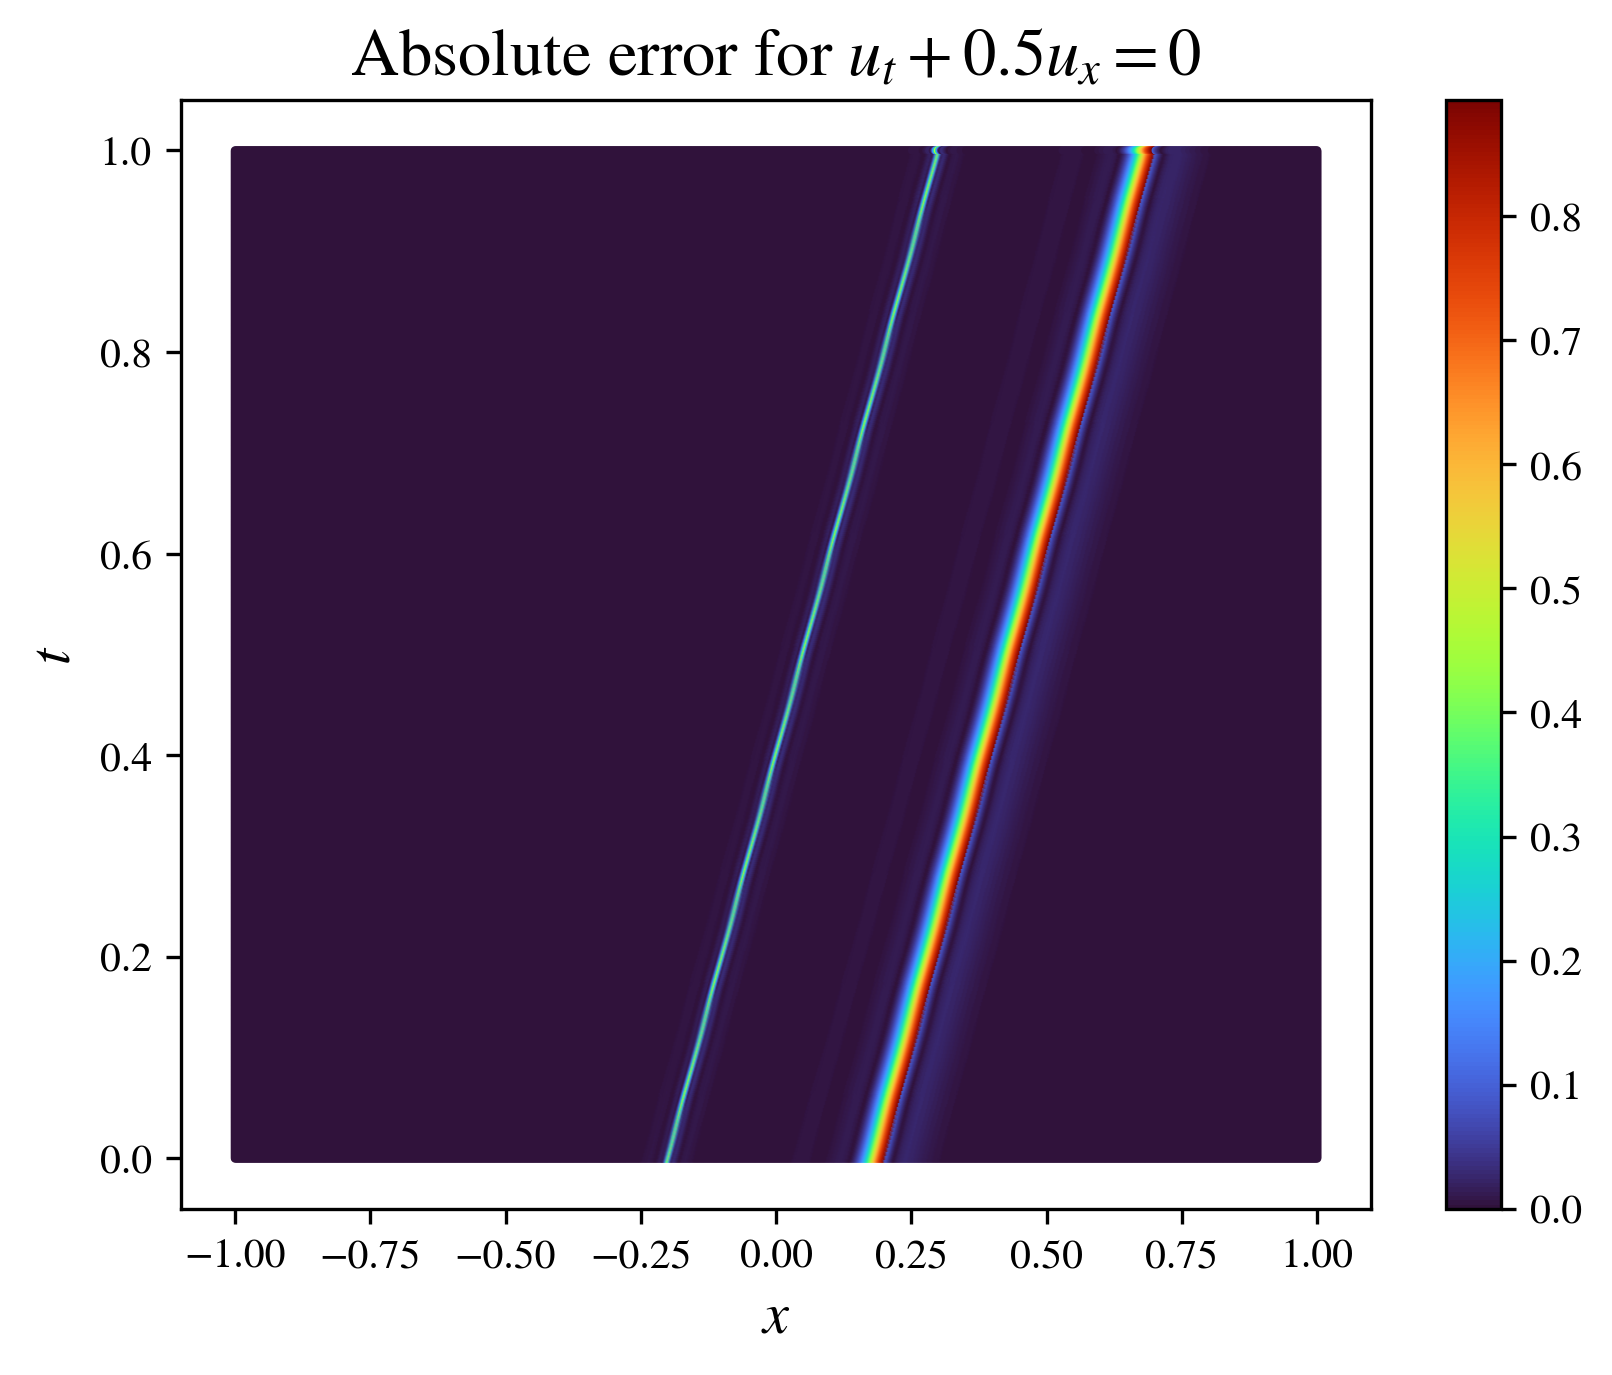
\includegraphics[width=0.8\linewidth]{Project1XPINNs/figures/advection/single_advection_error.png}
    \caption{Absolute errors against the true solution, with a single PINN.}
    \label{fig:single_ad_error}
\end{figure}

We stress test our model by changing the equation in question by setting $\alpha=-1$, while keeping the same domain decomposition.
This is done in order to ensure that the XPINN is not simply learning the domain decomposition, but rather the behaviour we are expecting.
The wave is now able to traverse across the subdomain decomposition, as in \autoref{fig:alpha-1_pred}, however with worse errors in \autoref{fig:alpha-1_error} than we saw previously.
This is a promising result before moving on to more difficult problems.

\begin{figure}[h!]
    \centering
    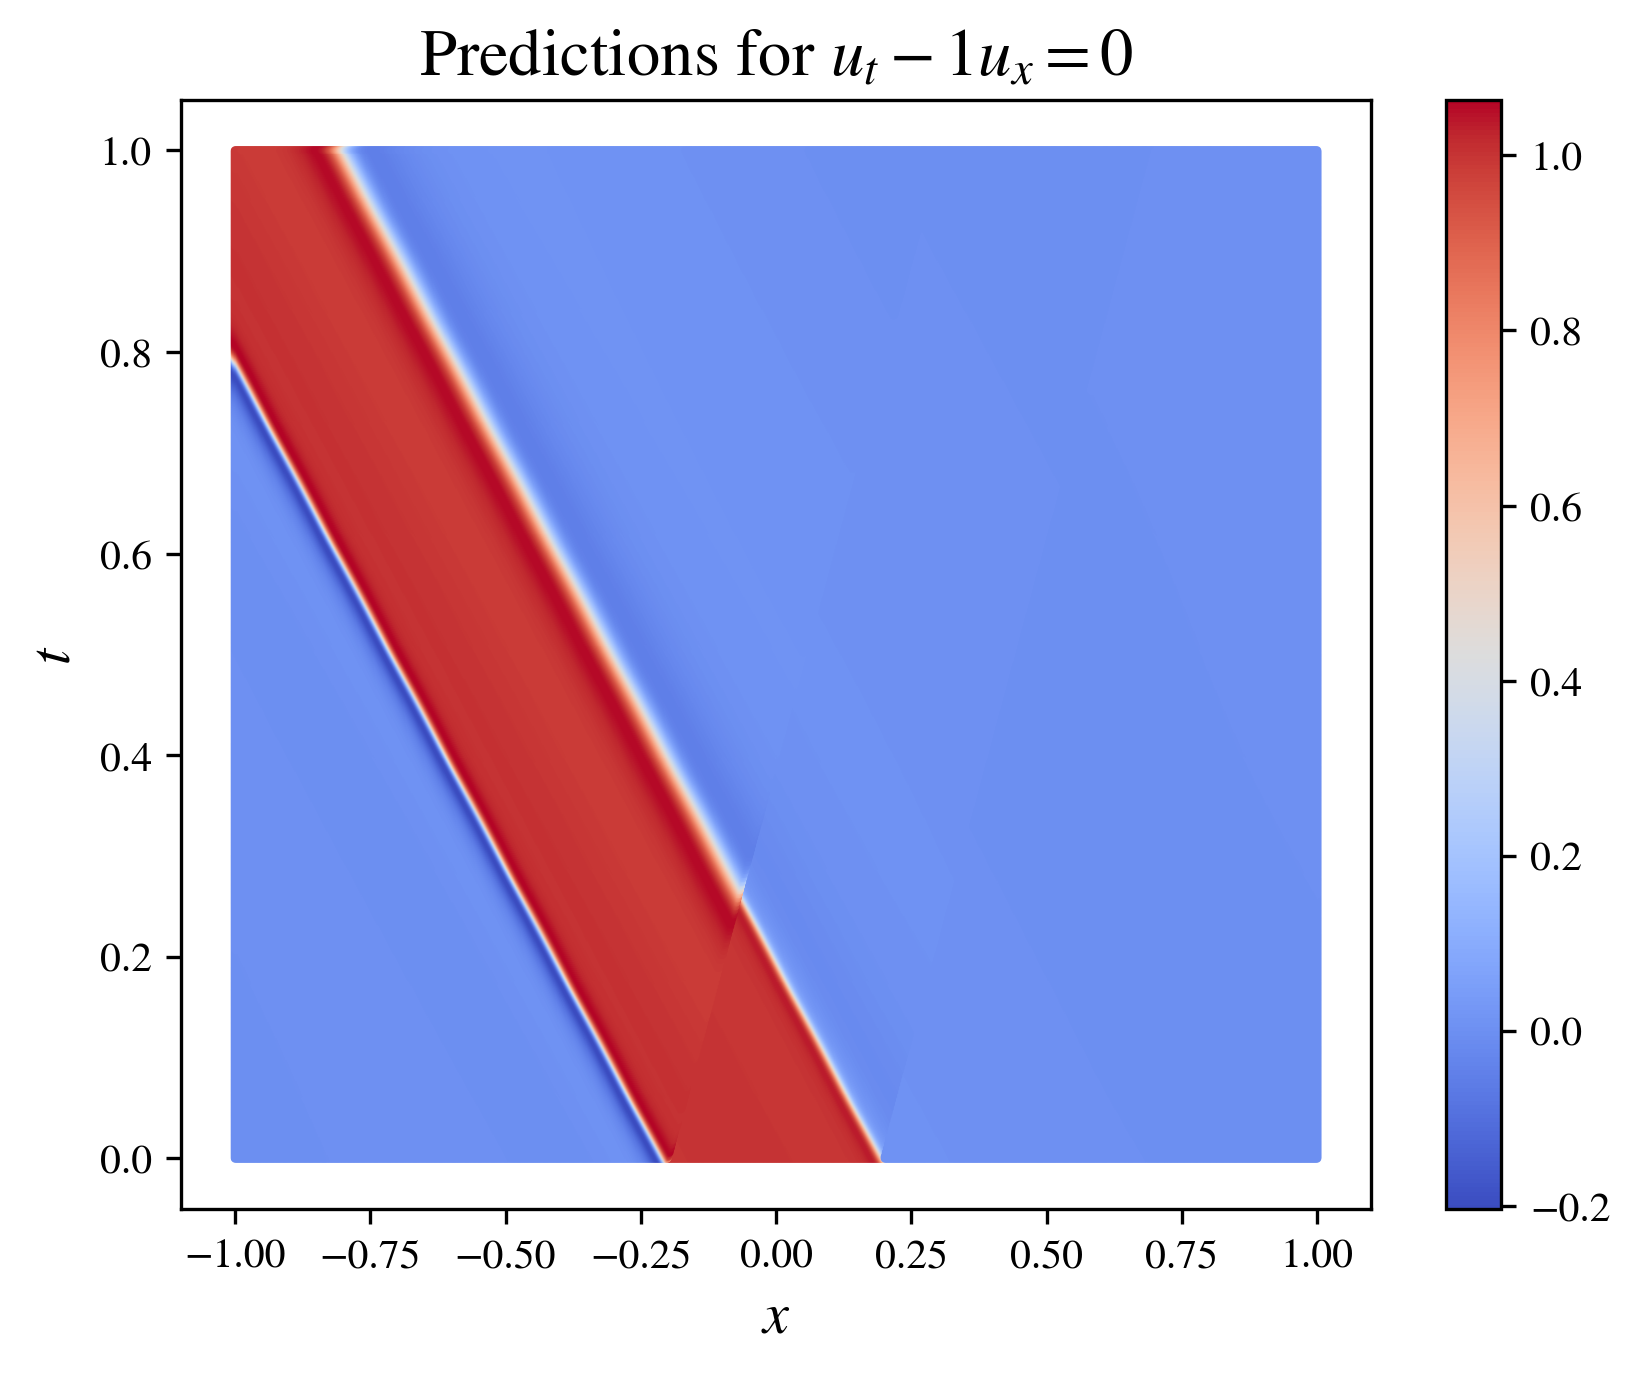
\includegraphics[width=0.8\linewidth]{Project1XPINNs/figures/advection/xpinn_stress_predictions.png}
    \caption{Predictions with $\alpha=-1$, same decomposition.}
    \label{fig:alpha-1_pred}
\end{figure}

\begin{figure}[h!]
    \centering
    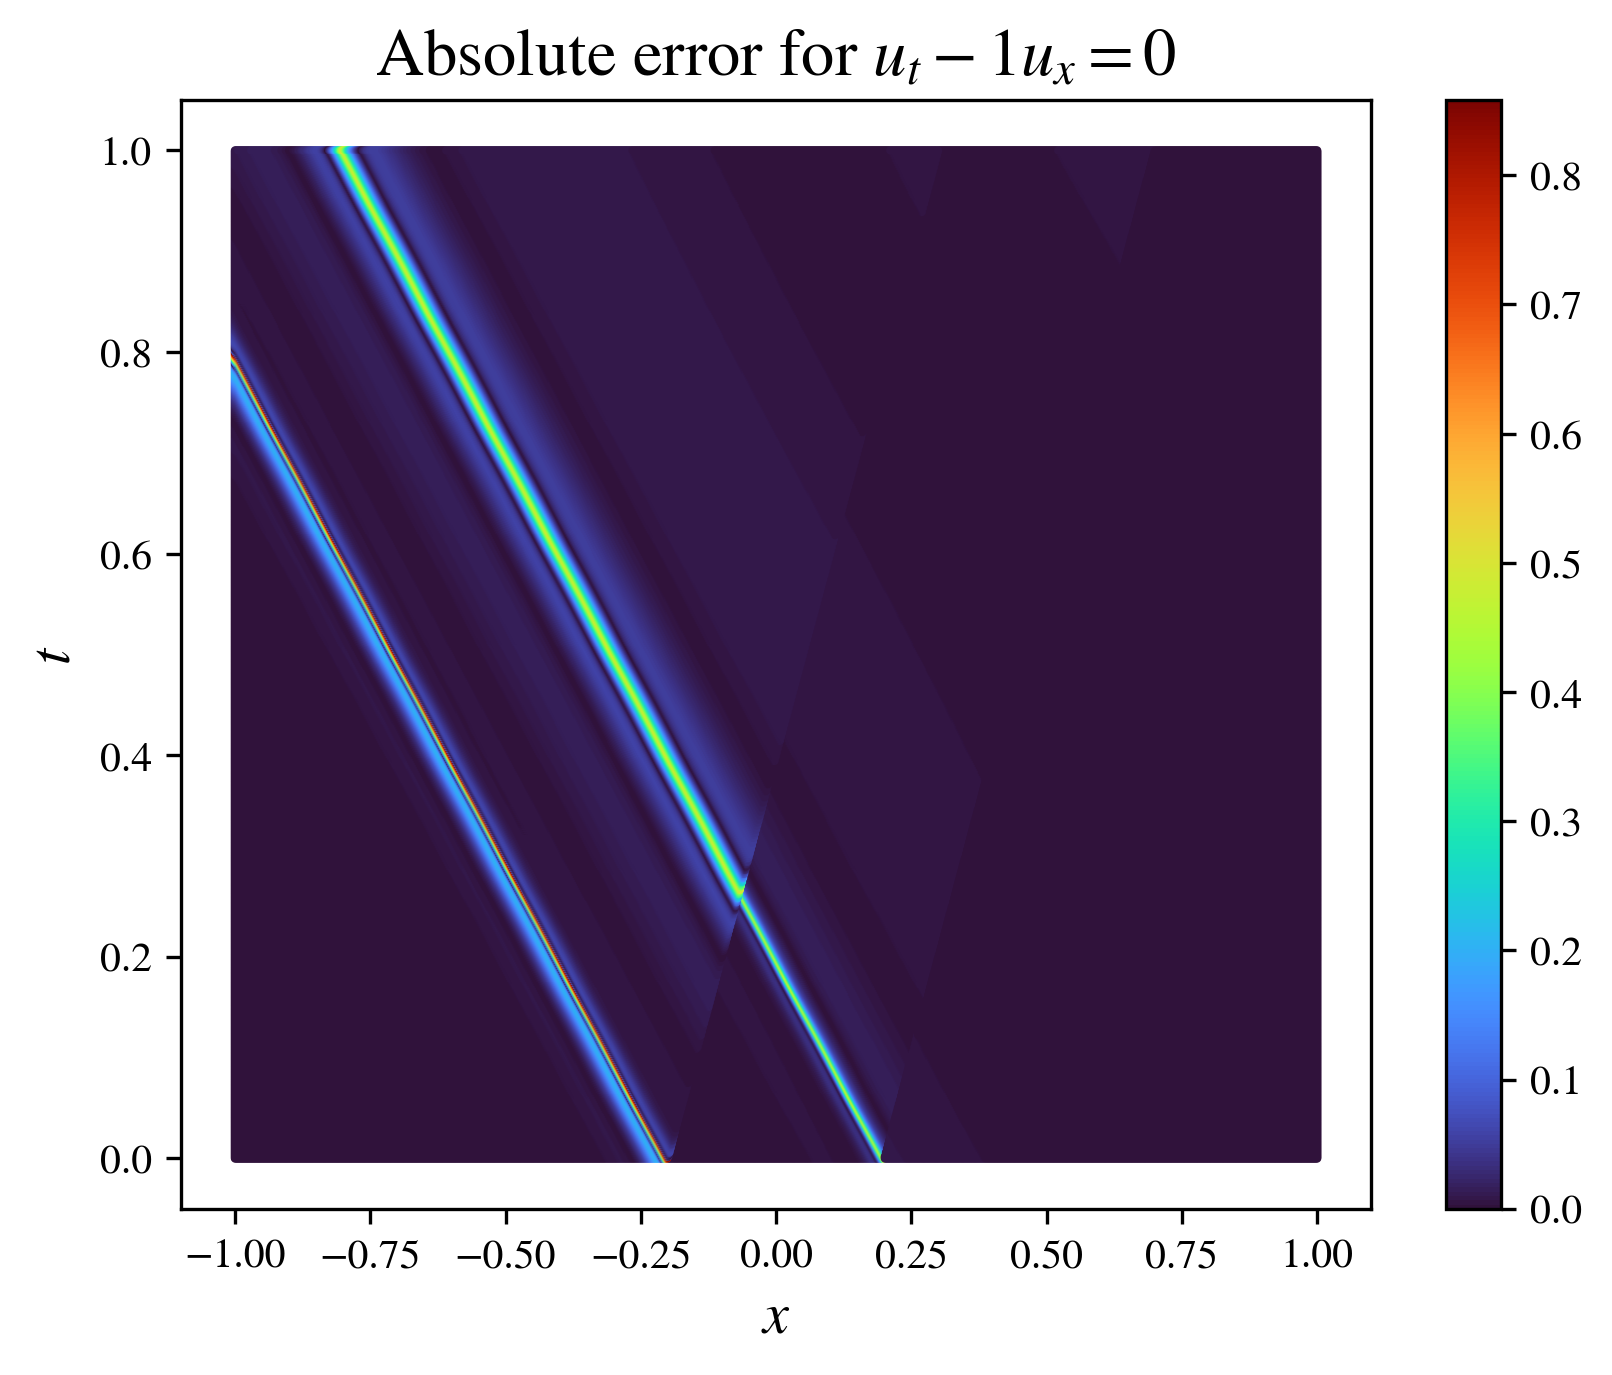
\includegraphics[width=0.8\linewidth]{Project1XPINNs/figures/advection/xpinn_stress_error.png}
    \caption{Absolute error with $\alpha=-1$.}
    \label{fig:alpha-1_error}
\end{figure}

% \vfill\null

\subsection{Poisson Equation}
\subsubsection{Problem Formulation}
In this subsection, we consider a two-dimensional Poisson equation with residual discontinuity.
The problem is a second order linear PDE, and is defined as
\begin{align}\label{eq:poisson}
\begin{cases}
    u_{xx}+u_{yy} = f &\text{on } \Omega \\
    u(x,y) = 0 &\text{on } \partial\Omega,
\end{cases}
\end{align}
where $\Omega = [0,1] \times [0,1]$.
For the Poisson equation, we consider two residuals.

\paragraph{Continuous Residual:}
The first residual is given by
\begin{equation}\label{eq:continuous_poisson}
    f_{\text{cont}}(x,y)= -2\pi^2\sin(\pi x) \sin(\pi y),
\end{equation}
which yields the known analytical solution
\begin{equation*}
    u_{\text{true}}(x,y)=\sin(\pi x) \sin(\pi y),
\end{equation*}
which is displayed in \autoref{fig:exact_smooth}.

\begin{figure}[h]
    \centering
    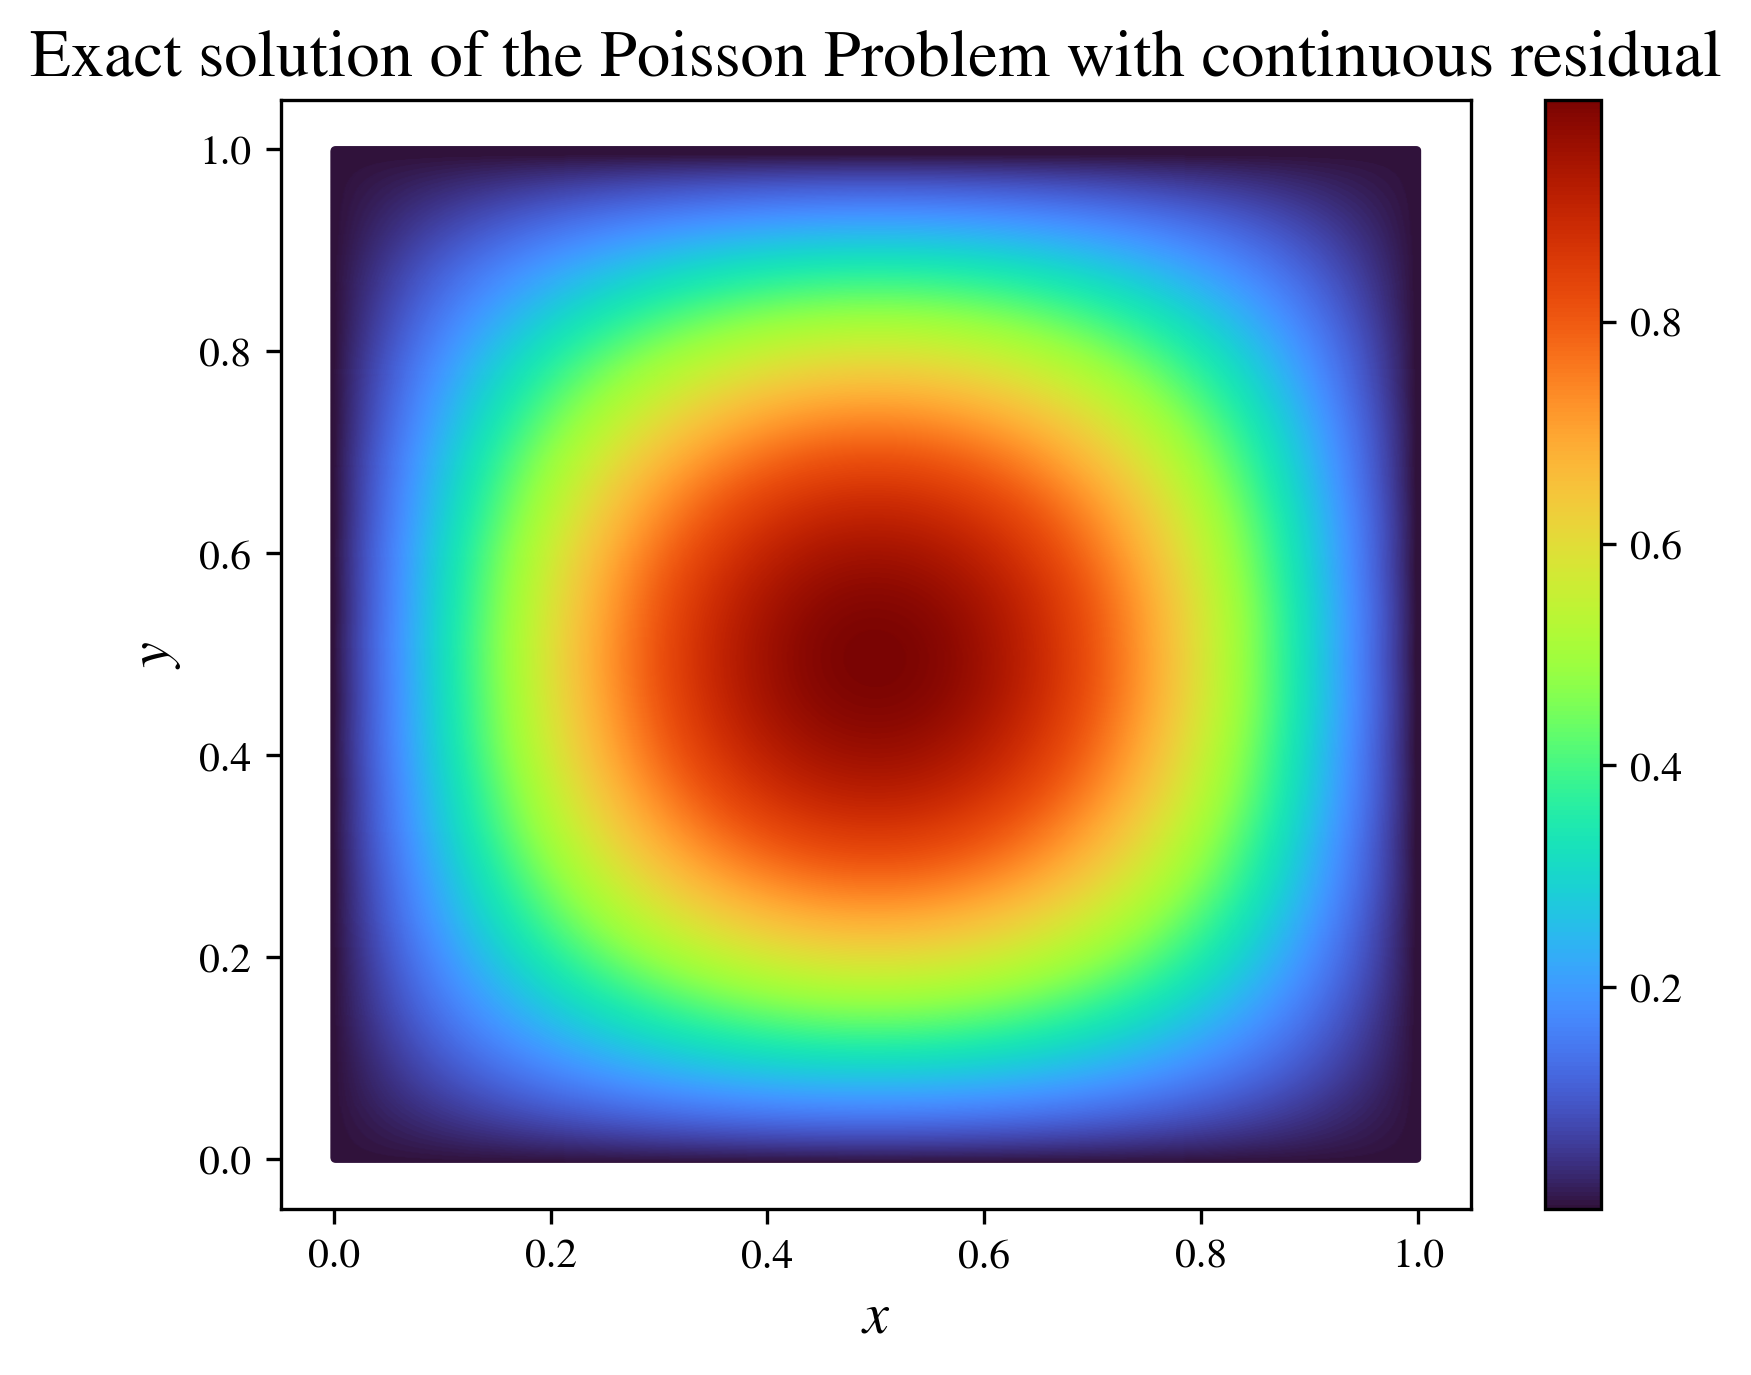
\includegraphics[width=0.8\linewidth]{Project1XPINNs/figures/Poisson/smooth_Poisson_true.png}
    \caption{The exact analytical solution to the Poisson equation with continuous residual.}
    \label{fig:exact_smooth}
\end{figure}

Our experimental setup follows that of \textcite{müller2023achieving}.
We consider the problem for both a single PINN and for an XPINN decomposition shown in \autoref{fig:decomp_poisson}.
For the PINN, we train using 900 interior points and 120 boundary points distributed uniformly.
For the XPINN, we also add 80 uniformly distributed interface points. Thus, the total amount of training points used for the XPINN exceeds that for the PINN.
We apply unitary weights to the different losses.
All PINNs have the same architecture of a 3-layered neural network with 64 hidden units, and we use the $\tanh$ activation function. 
Both solvers are trained using the \textsc{Adam} optimizer with an exponentially decreasing learning rate.
The initial learning rate is $10^{-3}$.
After $1.5\times 10^4$ steps, we decrease the learning rate by a factor of $10^{-1}$ every $10^4$ steps until a minimum learning rate of $10^{-7}$.
We train both cases for $2\times 10^5$ iterations. For our testing, we consider a uniform grid with 1 000 000 points. 

\begin{figure}[h]
    \centering
    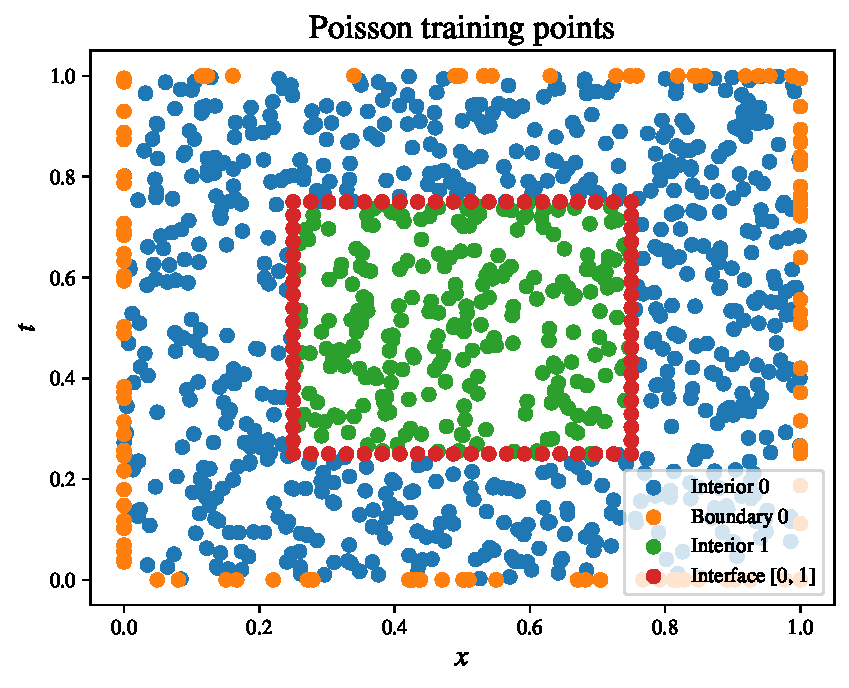
\includegraphics[width=0.8\linewidth]{Project1XPINNs/figures/Poisson/poisson_train_points.pdf.pdf}
    \caption{Training points with the XPINN decomposition for the Poisson equation. The PINN is given the same points, without the interface points.}
    \label{fig:decomp_poisson}
\end{figure}

\paragraph{Discontinuous Residual:}
The second residual is due \textcite{XPINN_generalize}, where they compare the generalizeability of PINNs and XPINNs.
The residual is given as a discontinuous form
\begin{equation*}\label{eq:discontinuous_poisson}
    f_{disc}(x,y)=
    \begin{cases}
        1 &\text{if} \, (x,y)\in [0.25,0.75]\times[0.25,0.75], \\
        0 &\text{else}.
    \end{cases}
\end{equation*}
The reference solution is computed numerically using the \verb|poissonpy| package \cite{poissonpy} on the uniform test mesh with 1 000 000 points, displayed in \autoref{fig:exact_discontinuous}.
We apply a 9 layer neural network with 20 hidden units, using the $\tanh$ activation function.
Again, we apply 900 internal, 120 boundary and 80 interface points for training the XPINN model, as in \autoref{fig:decomp_poisson}.
\textsc{Adam} is again used with the same exponential decay rate, and the solvers are run for $2\times 10^5$ iterations.
Note that the paper by \textcite{XPINN_generalize} uses the LBFGS optimizer, however this is currently unavailable in \verb|optax| as it is under development. Implementing LBFGS from scratch without \verb|optax| is outside the scope of this project as it would make our implementation less comparable to our other \verb|optax| methods.

\begin{figure}[h]
    \centering
    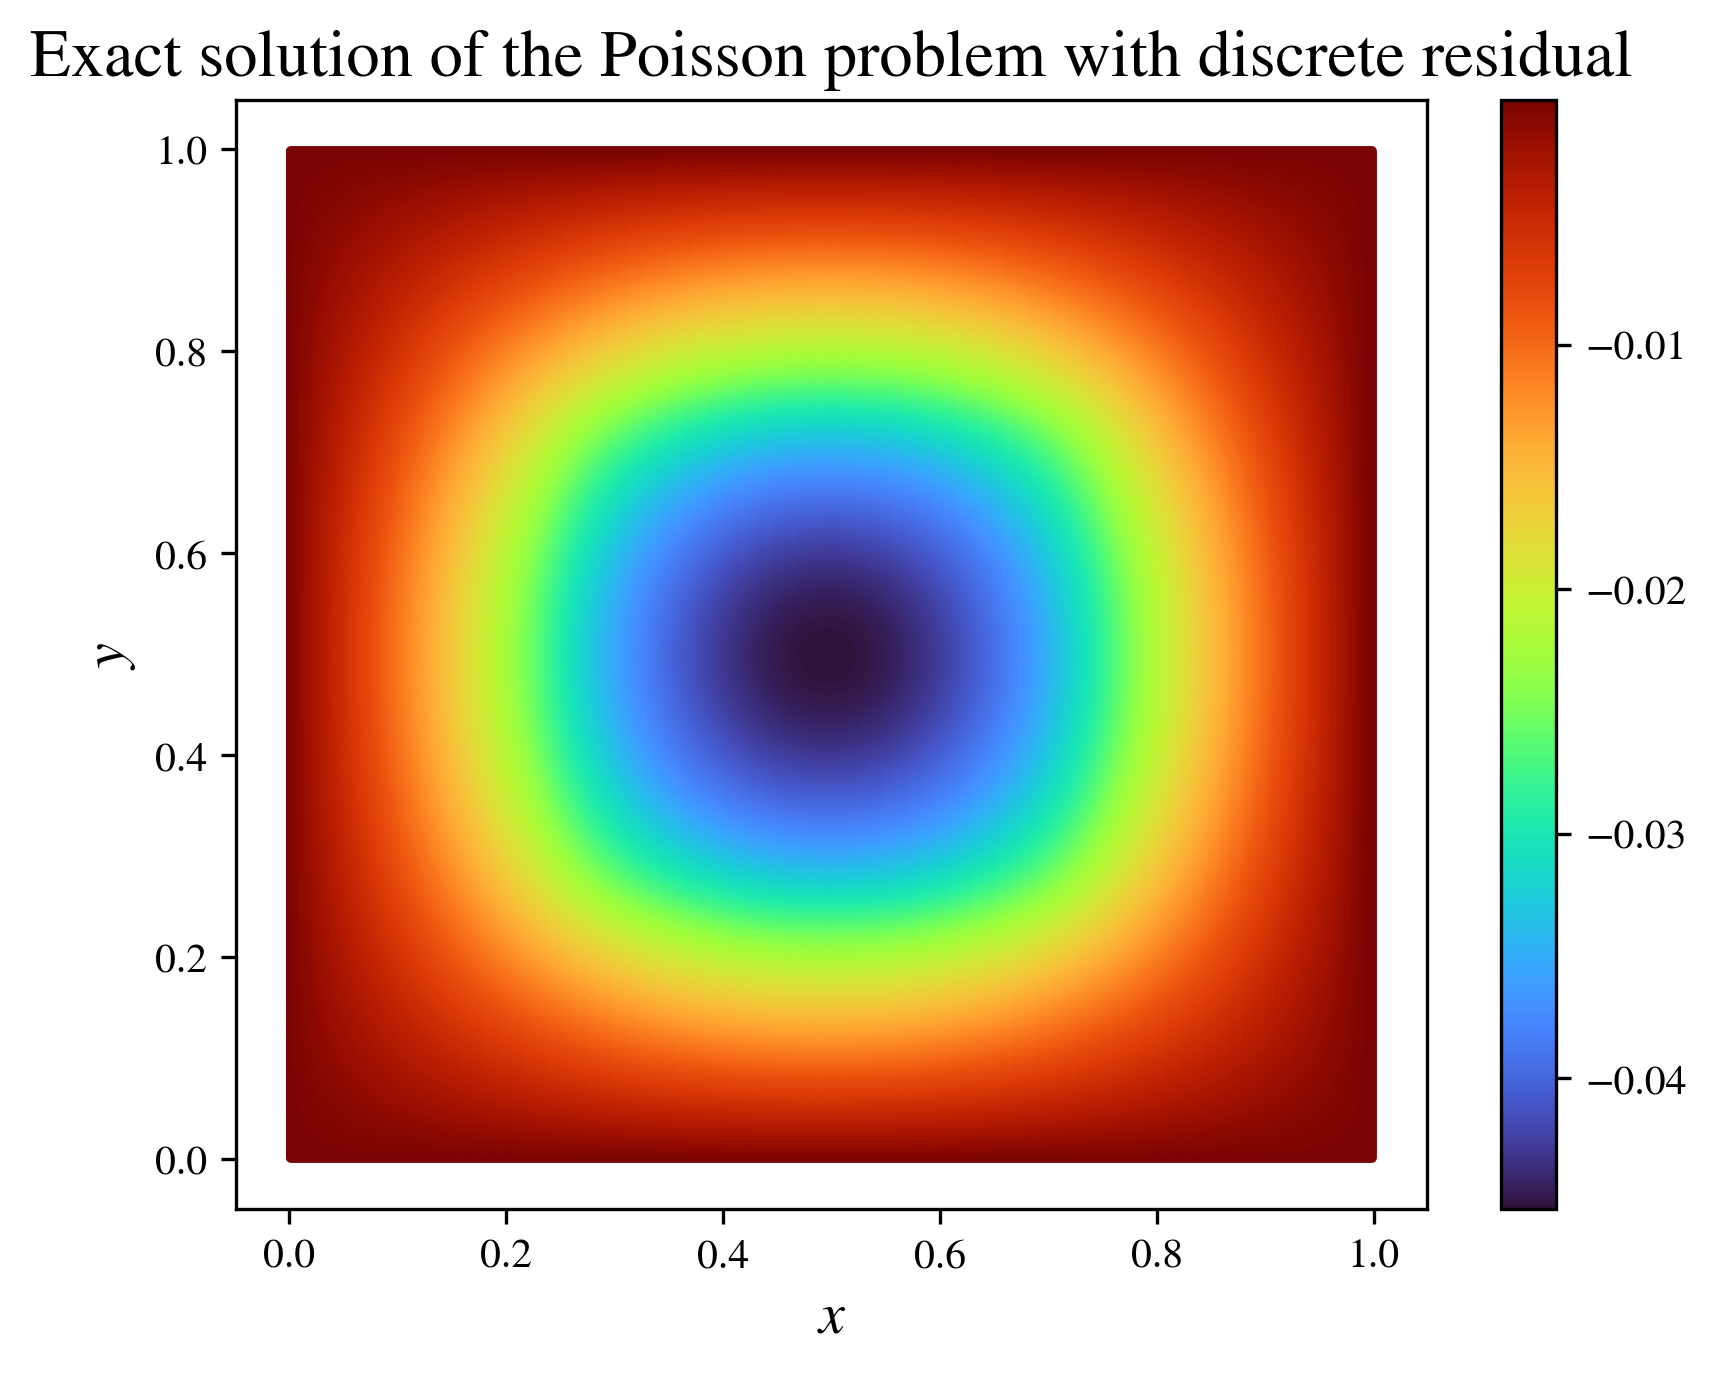
\includegraphics[width = 0.7\linewidth]{Project1XPINNs/figures/Poisson/discrete_Poisson_solution.png}
    \caption{Numerically computed reference solution to the Poisson equation with discontinuous residual.}
    \label{fig:exact_discontinuous}
\end{figure}

\subsubsection{Results}
\paragraph{Continuous Residual:}
\autoref{table:cont_poisson} shows the minimum, median, and maximum relative $L^2$ errors of the single PINN and XPINN solvers for the continuous residual Poisson equation using the \textsc{Adam} optimizer, across ten iterations.
Note that the training mesh was re-generated between each iteration.

% \vfill\null

\autoref{fig:rel_l2_smooth_poisson} displays the $L^2$ error evolution against the iterations.
From the figure, we see that the $L^2$ error seems to stabilize.
Although of similar orders of magnitude, we see that the PINN model frequently outperforms our XPINN discretization.
This is as expected by the argument of \textcite{XPINN_generalize}, as the domain decomposition does not reduce the target function complexity in the subdomains, whereas each subdomain trains on fewer points than the PINN. 

\begin{table}[h]
\caption{Median, minimum and maximum of the relative $L^2$-errors for the Poisson equation with continuous residual achieved by the PINN and XPINN.}
    \centering
    \begin{tabular}{r|c|c|c}\toprule
     & Median & Minimum & Maximum
    \\
    \colrule
    PINN & $1.37\cdot 10^{-3}$ &  $8.4 \cdot 10^{-4}$ & $2.16 \cdot 10^{-3}$ 
    \\
    XPINN & $2.82\cdot 10^{-3} $ &  $1.23 \cdot 10^{-3}$ & $5.42 \cdot 10^{-3}$
    \\
    \botrule
    \end{tabular}
    \label{table:cont_poisson}
\end{table}

\begin{figure}[h!]
    \centering
    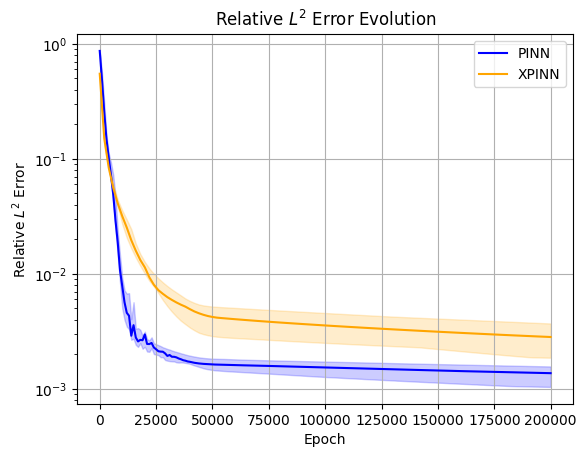
\includegraphics[width = 0.8\linewidth]{Project1XPINNs/figures/Poisson/Relative_L2_smooth_Adam.png}
    \caption{Relative $L^2$ error with median and interquartile range highlighted, for PINN and XPINN.}
    \label{fig:rel_l2_smooth_poisson}
\end{figure}

The PINN and XPINN predictions are shown in \autoref{fig:pinn_smooth_pred} and \autoref{fig:xpinn_smooth_pred}, and although they are hard to distinguish visually, the errors displayed in \autoref{fig:pinn_smooth_error} and \autoref{fig:xpinn_smooth_error} tell a different story.
We note that the significant sources of error for the PINN appear to be surrounding the boundaries.
The XPINN solution also shows boundary error, but is mainly dominated by the interface error.
Optimizing for the different weighting hyper-parameters might lowered the interface error, potentially at the cost of increased boundary error.

\begin{figure}[h]
    \centering
    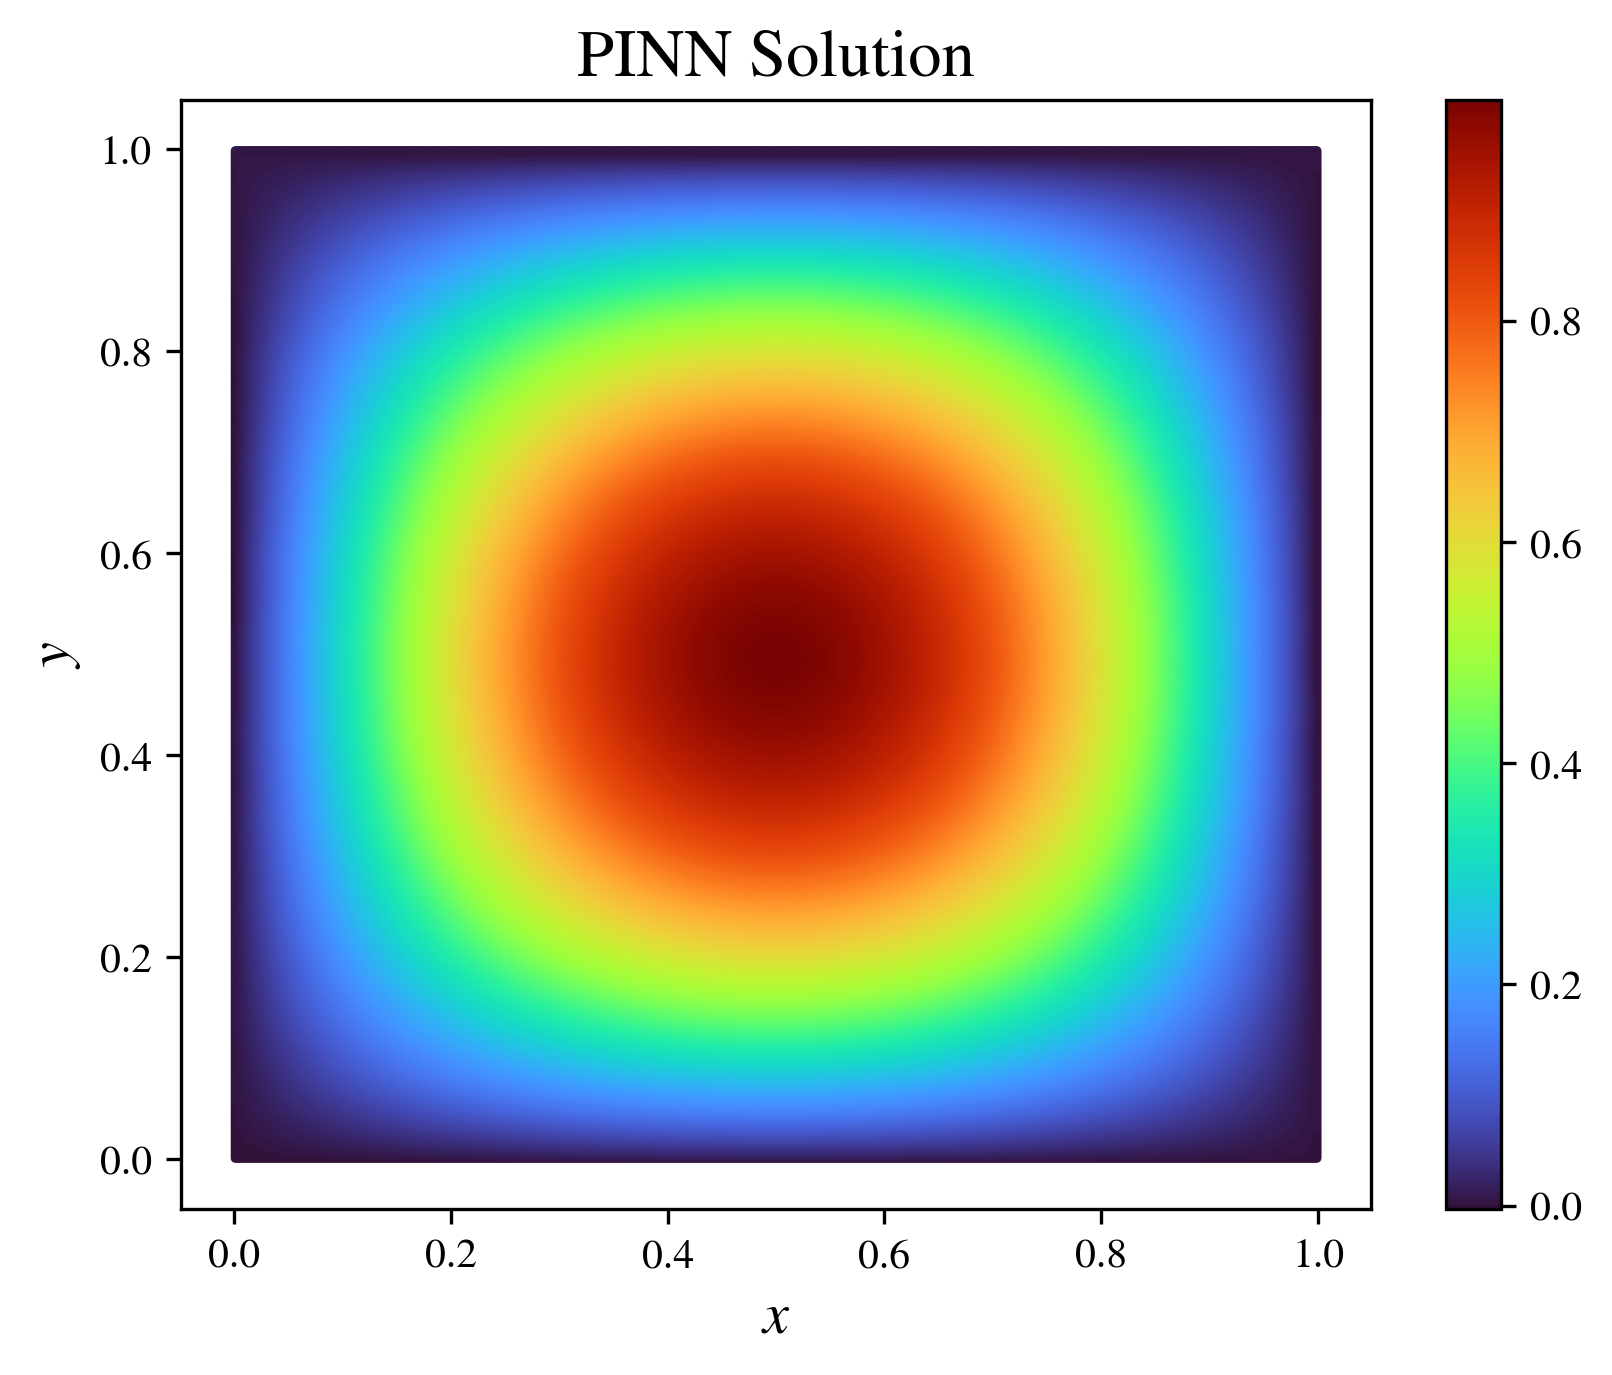
\includegraphics[width=0.7\linewidth]{Project1XPINNs/figures/Poisson/smooth_single_Poisson_solution.png}
    \caption{PINN prediction with continuous residual.}
    \label{fig:pinn_smooth_pred}
\end{figure}

\begin{figure}[h]
    \centering
    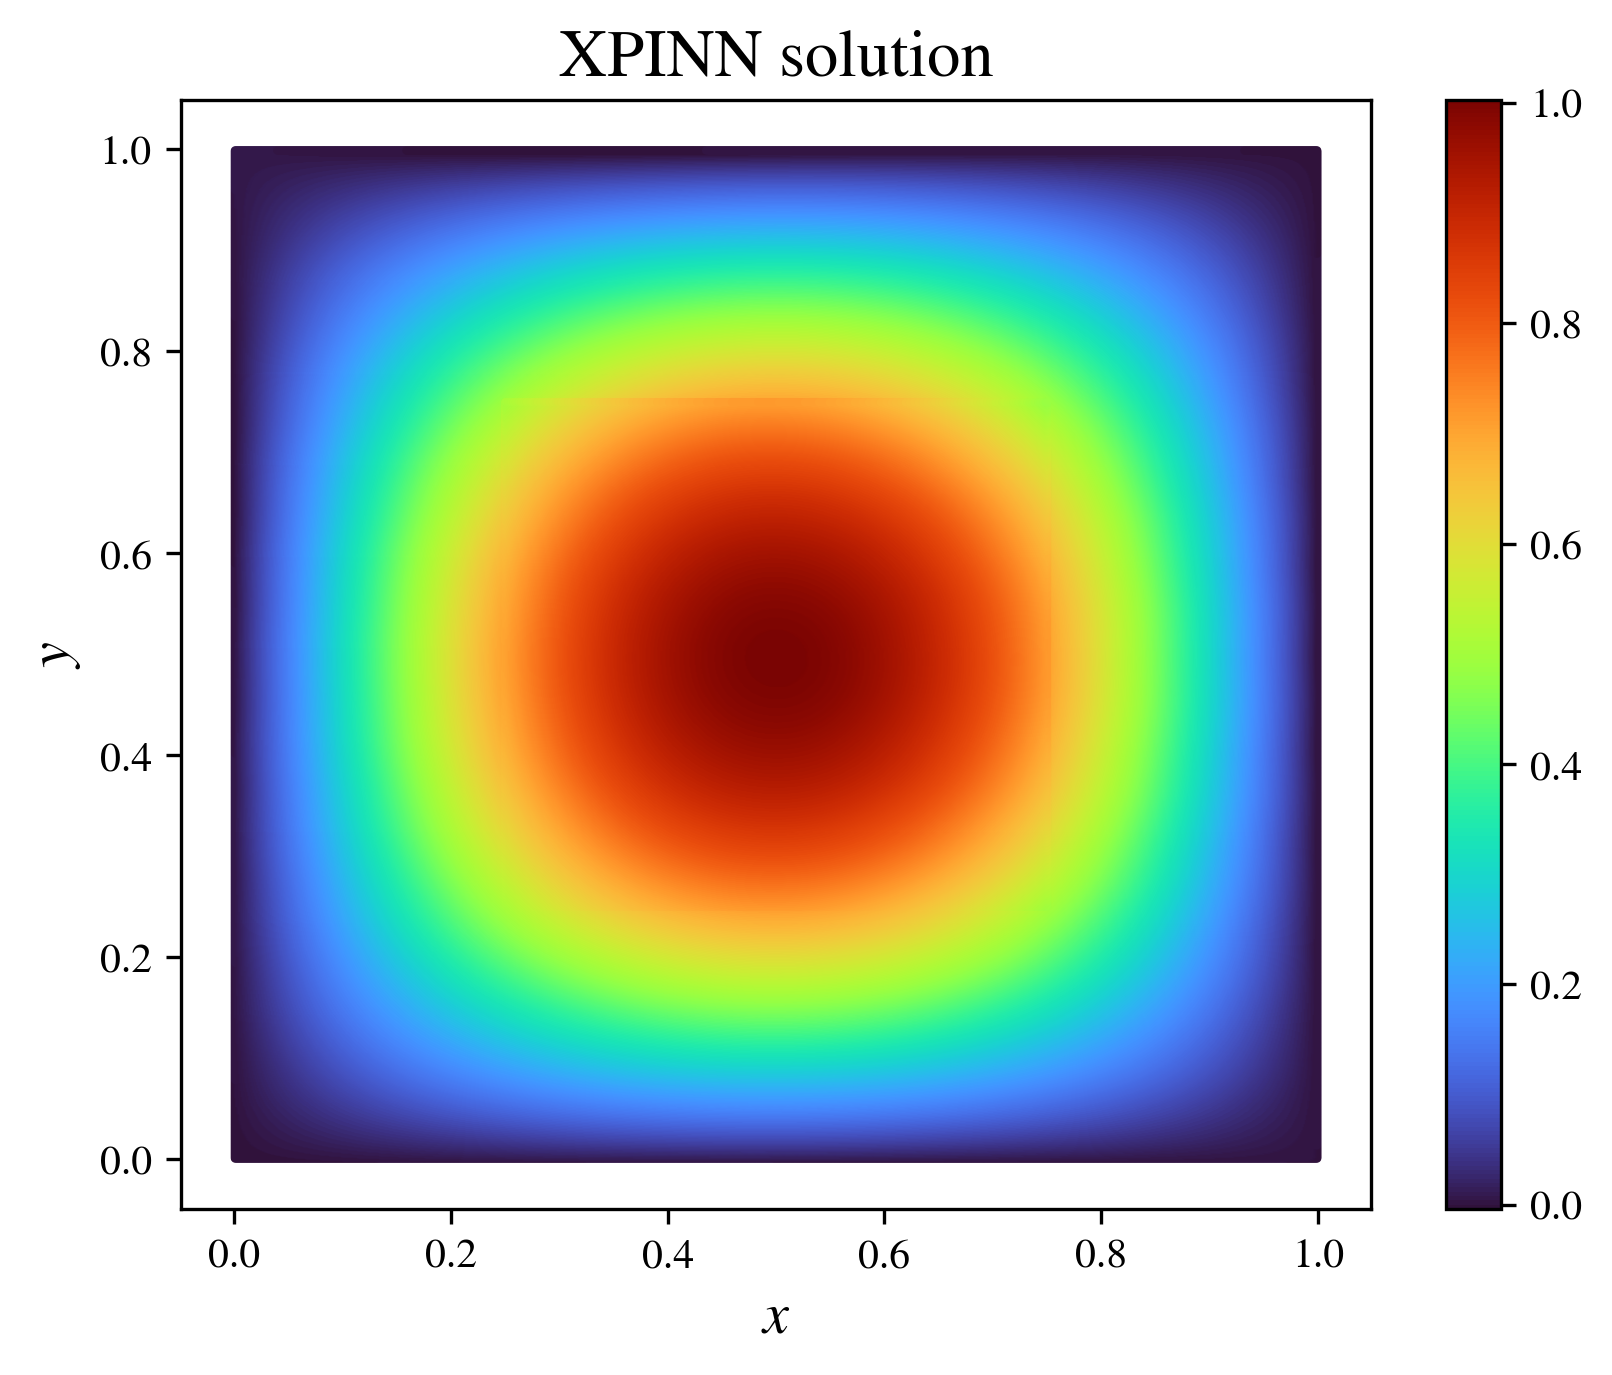
\includegraphics[width=0.7\linewidth]{Project1XPINNs/figures/Poisson/smooth_xpinn_Poisson_solution.png}
    \caption{XPINN prediction with continuous residual.}
    \label{fig:xpinn_smooth_pred}
\end{figure}

\begin{figure}[h]
    \centering
    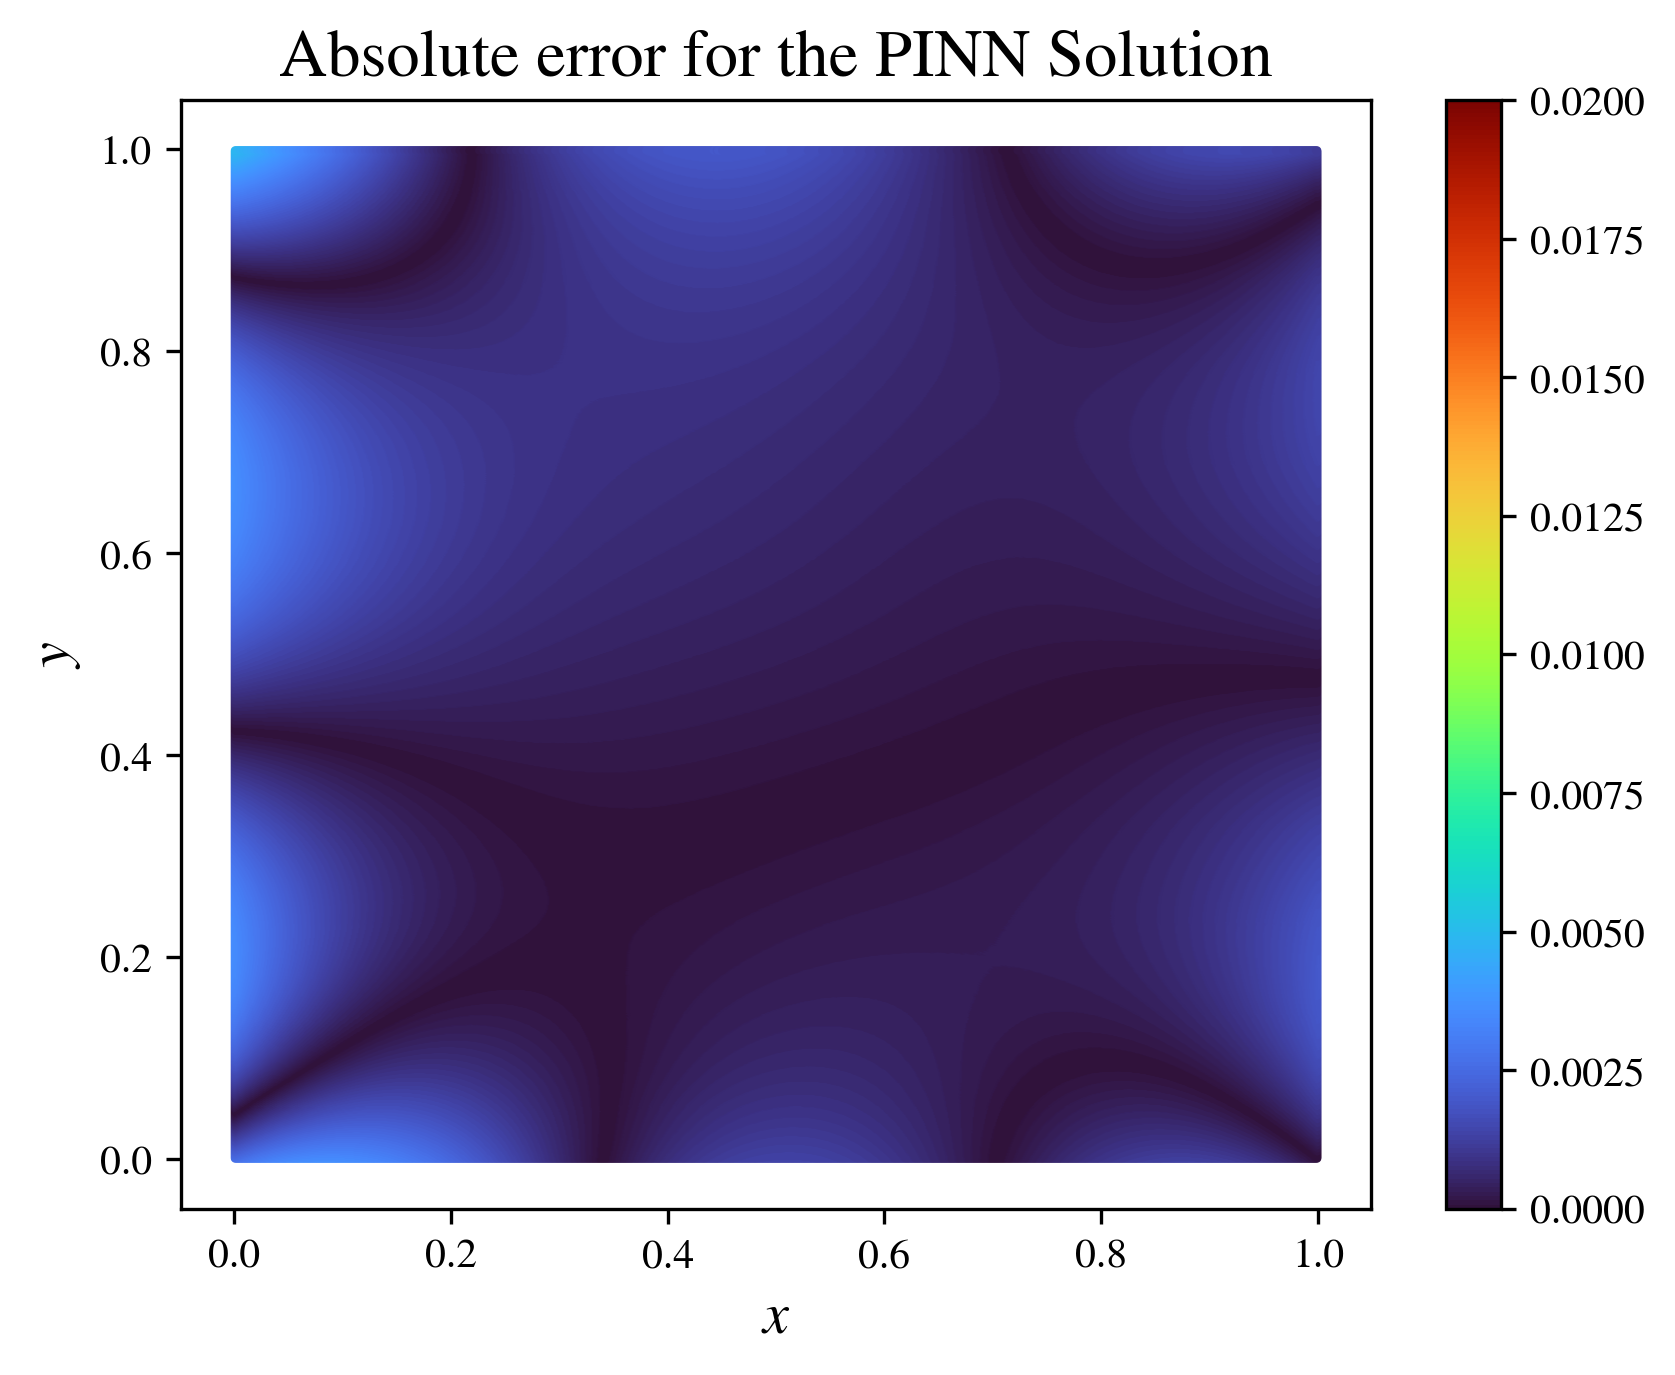
\includegraphics[width=0.7\linewidth]{Project1XPINNs/figures/Poisson/smooth_single_Poisson_error.png}
    \caption{PINN absolute error with continuous residual.}
    \label{fig:pinn_smooth_error}
\end{figure}

\begin{figure}[h]
    \centering
    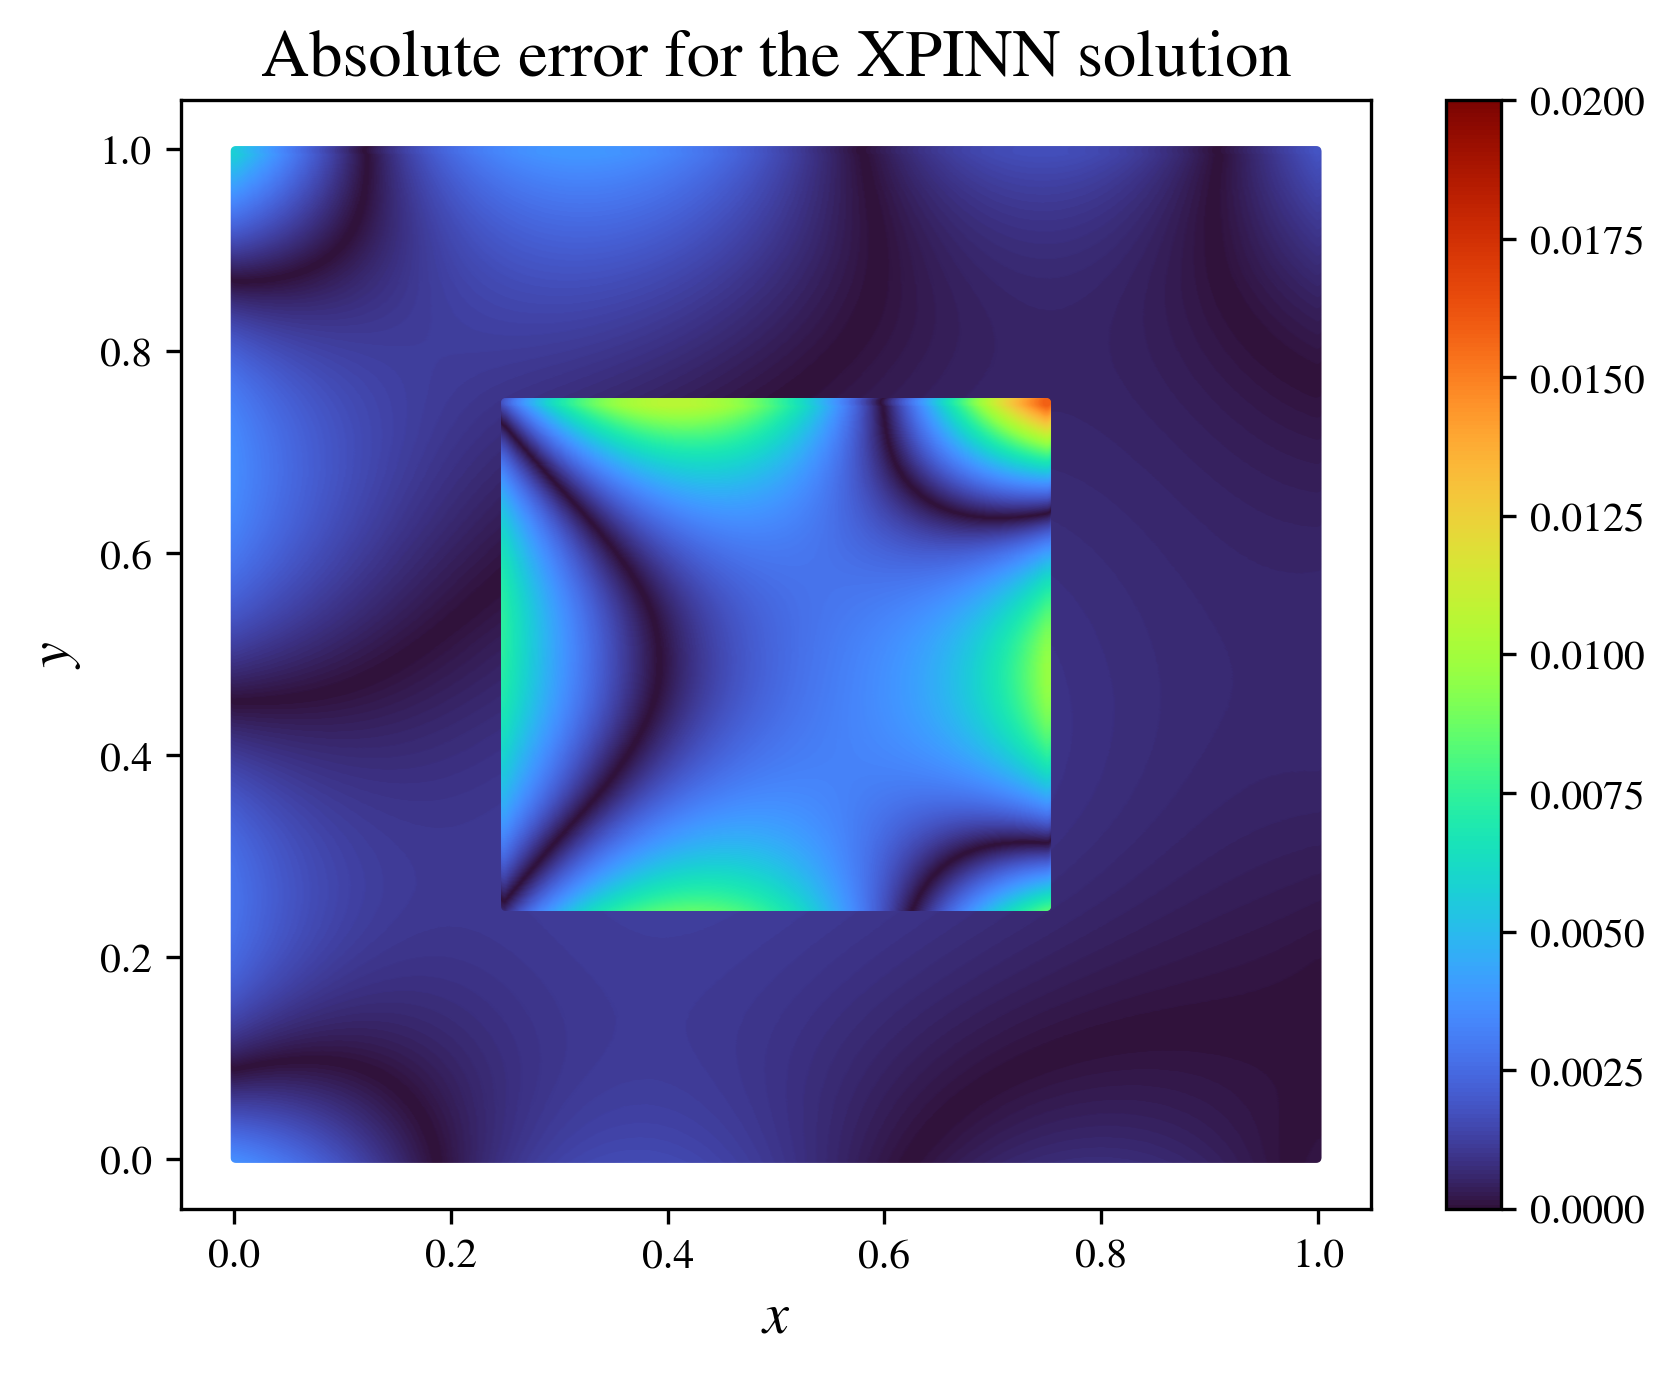
\includegraphics[width=0.7\linewidth]{Project1XPINNs/figures/Poisson/smooth_xpinn_Poisson_error.png}
    \caption{XPINN absolute error with continuous residual.}
    \label{fig:xpinn_smooth_error}
\end{figure}

% \vfill\null

\paragraph{Discontinuous Residual:}
\autoref{fig:pinn_disc_pred} and \autoref{fig:xpinn_disc_pred} display the PINN and XPINN solutions, alongside their errors on the domain, shown in \autoref{fig:pinn_disc_error} and \autoref{fig:xpinn_disc_error}.
Both solvers seem to perform worse on this problem. Notably, the XPINN solver appears to perform significantly worse, which is according to expectations \cite{XPINN_generalize}.

\begin{figure}[h]
    \centering
    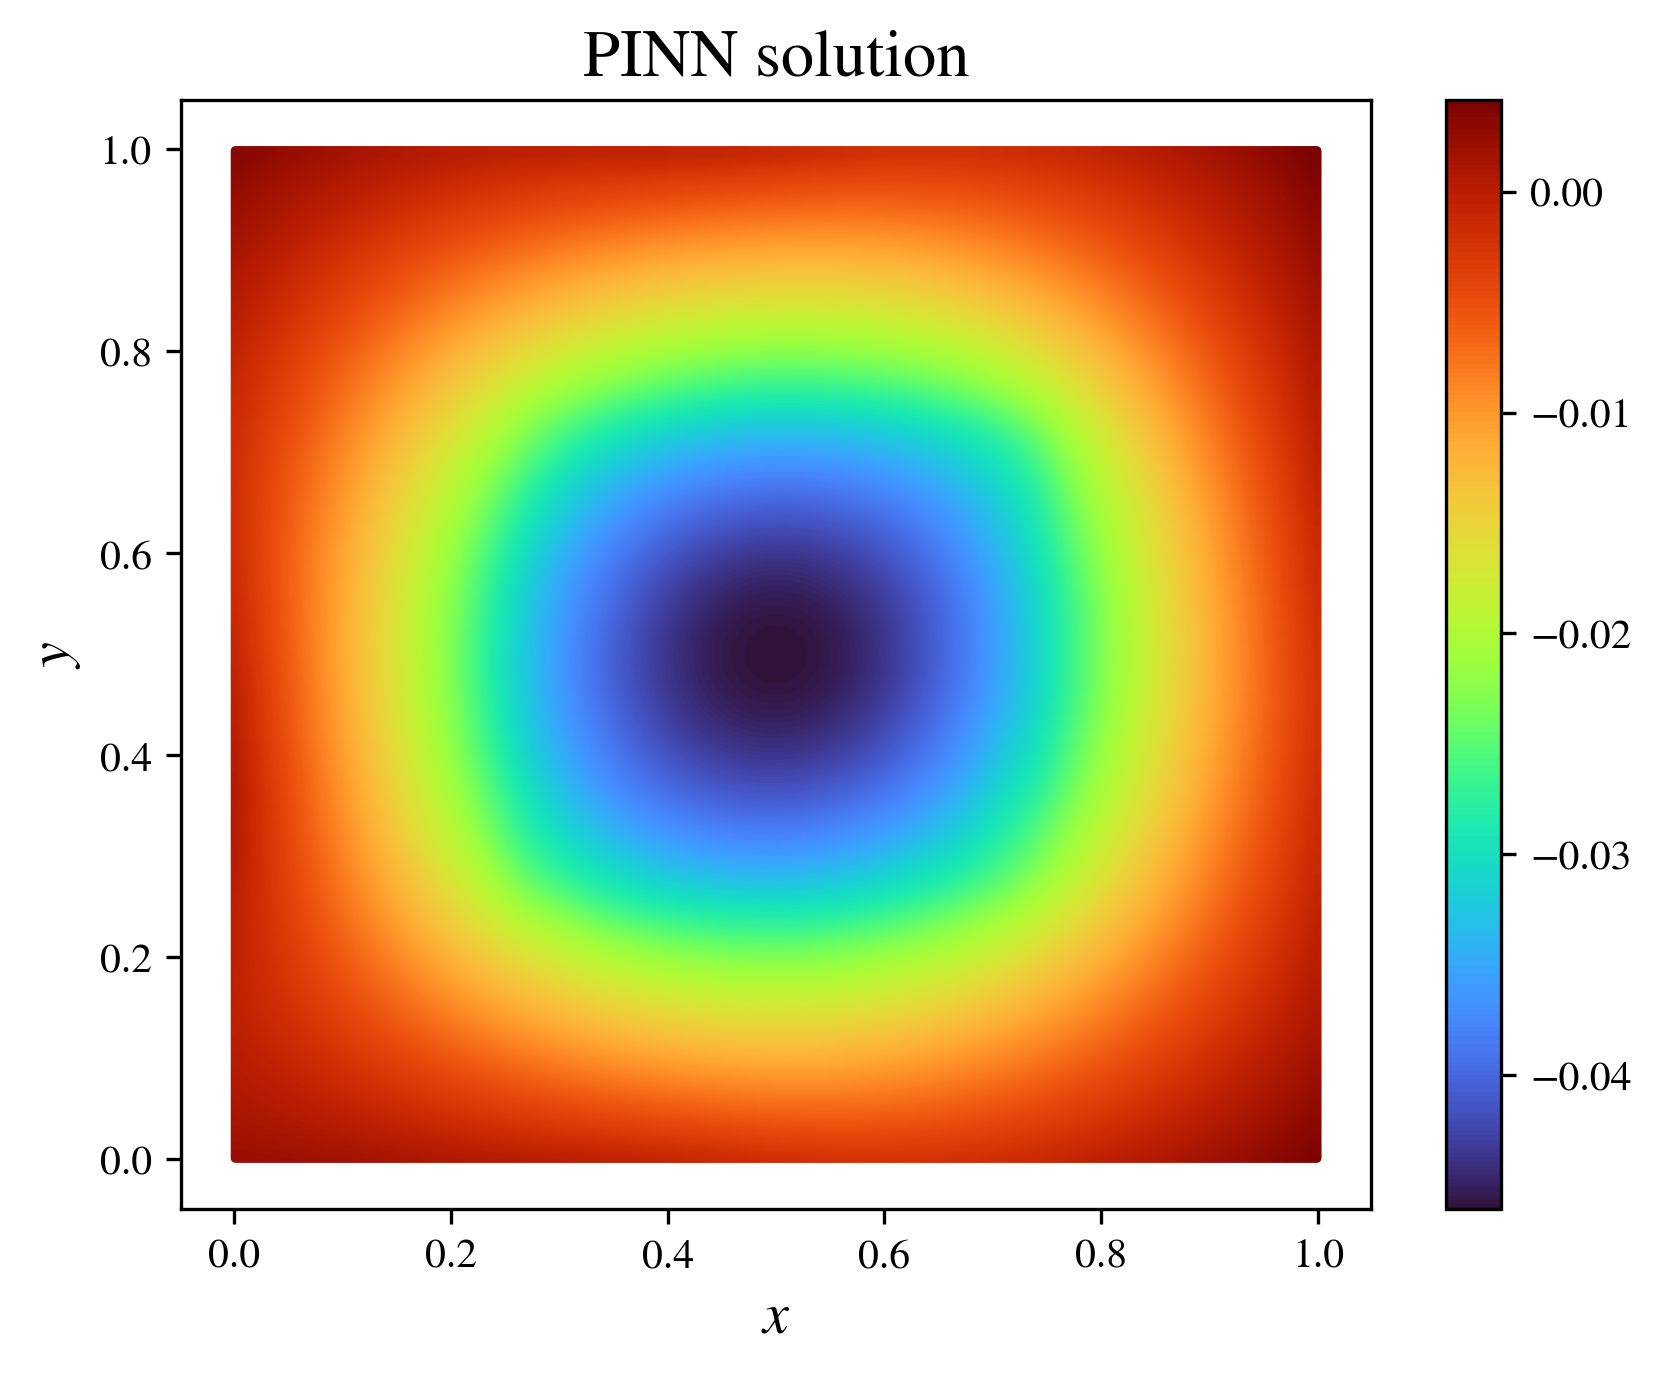
\includegraphics[width=0.7\linewidth]{Project1XPINNs/figures/Poisson/discrete_single_Poisson_solution.pdf.png}
    \caption{PINN prediction with discontinuous residual.}
    \label{fig:pinn_disc_pred}
\end{figure}

\begin{figure}[h]
    \centering
    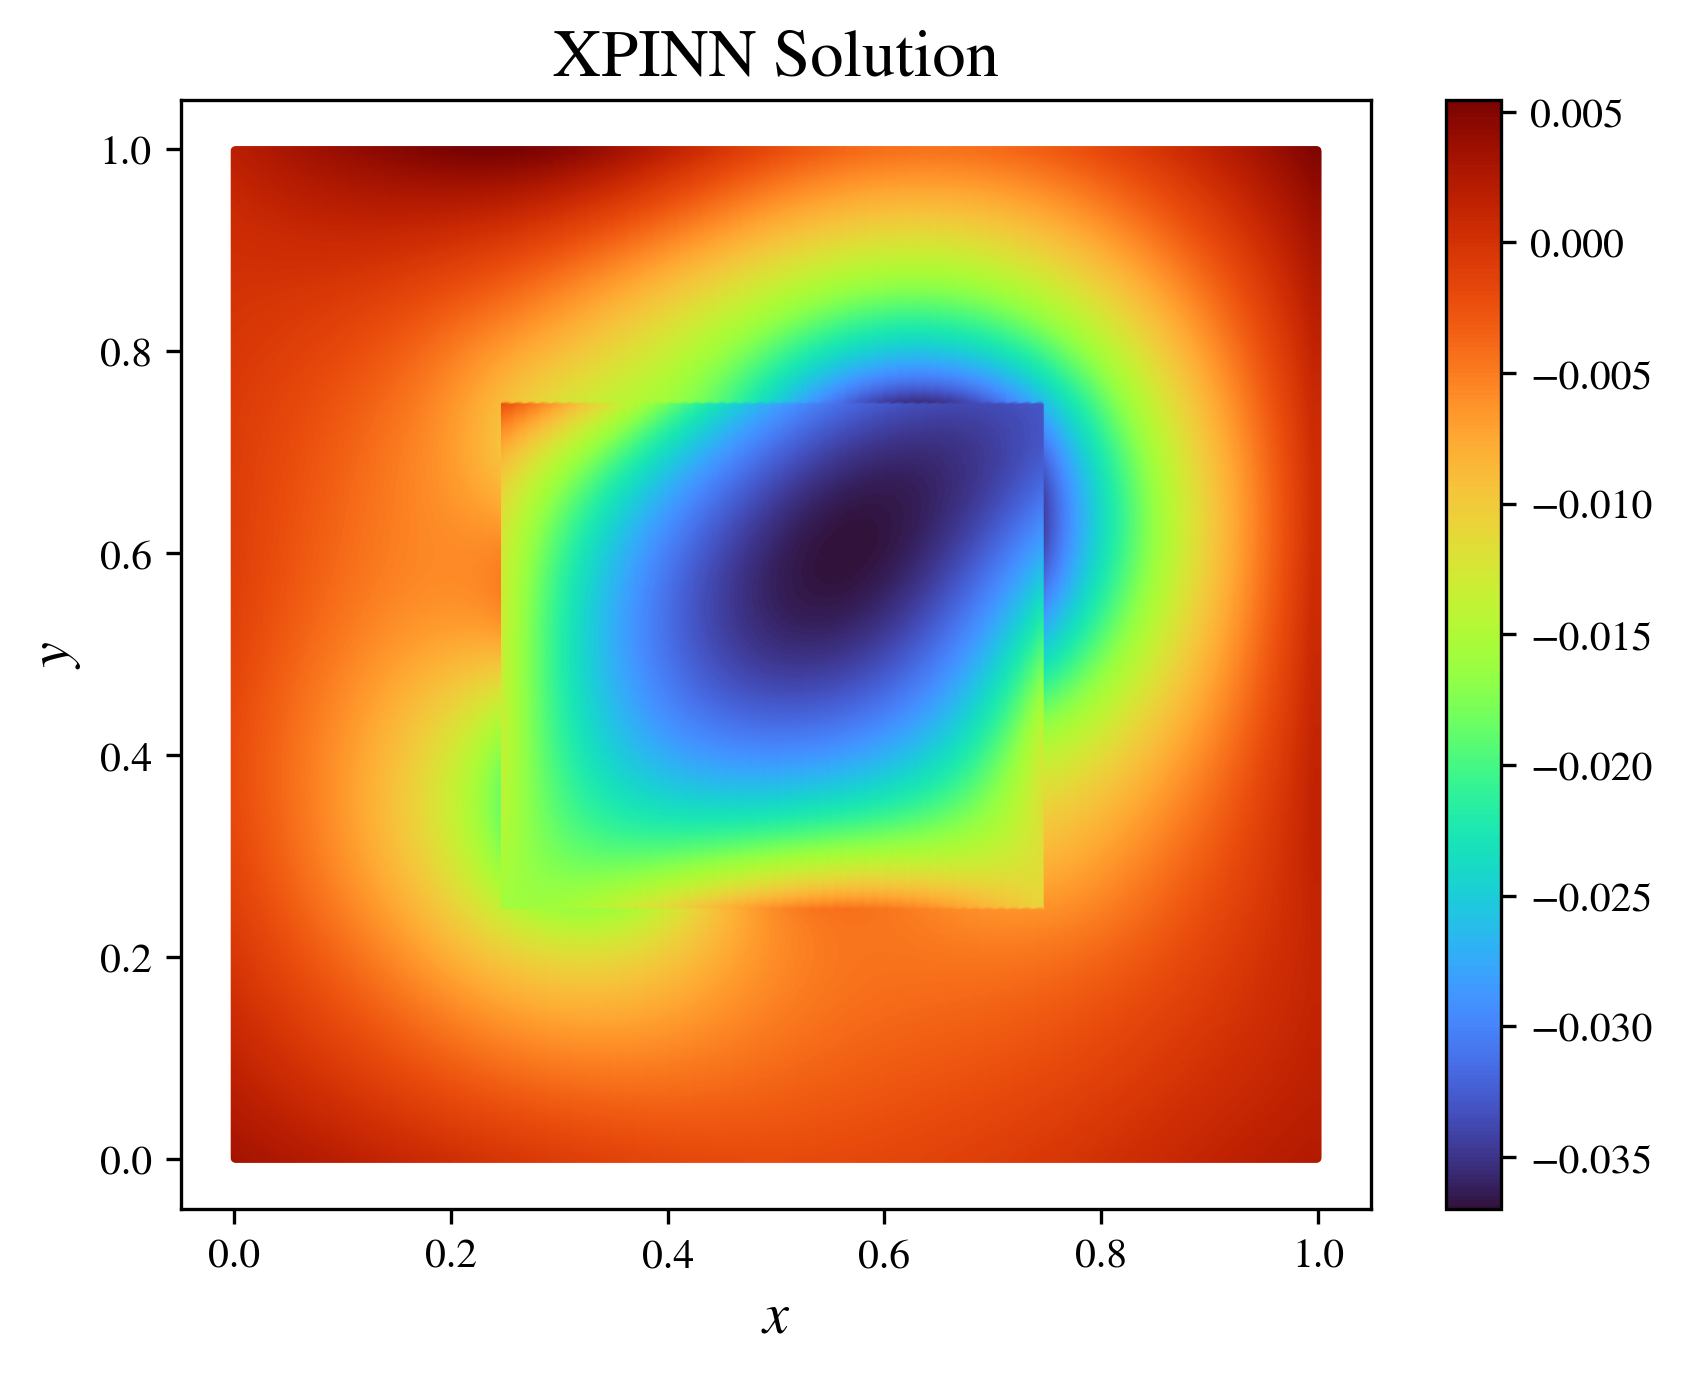
\includegraphics[width=0.7\linewidth]{Project1XPINNs/figures/Poisson/discrete_xpinn_Poisson_solution.png}
    \caption{XPINN prediction with continuous residual.}
    \label{fig:xpinn_disc_pred}
\end{figure}

\begin{figure}[h]
    \centering
    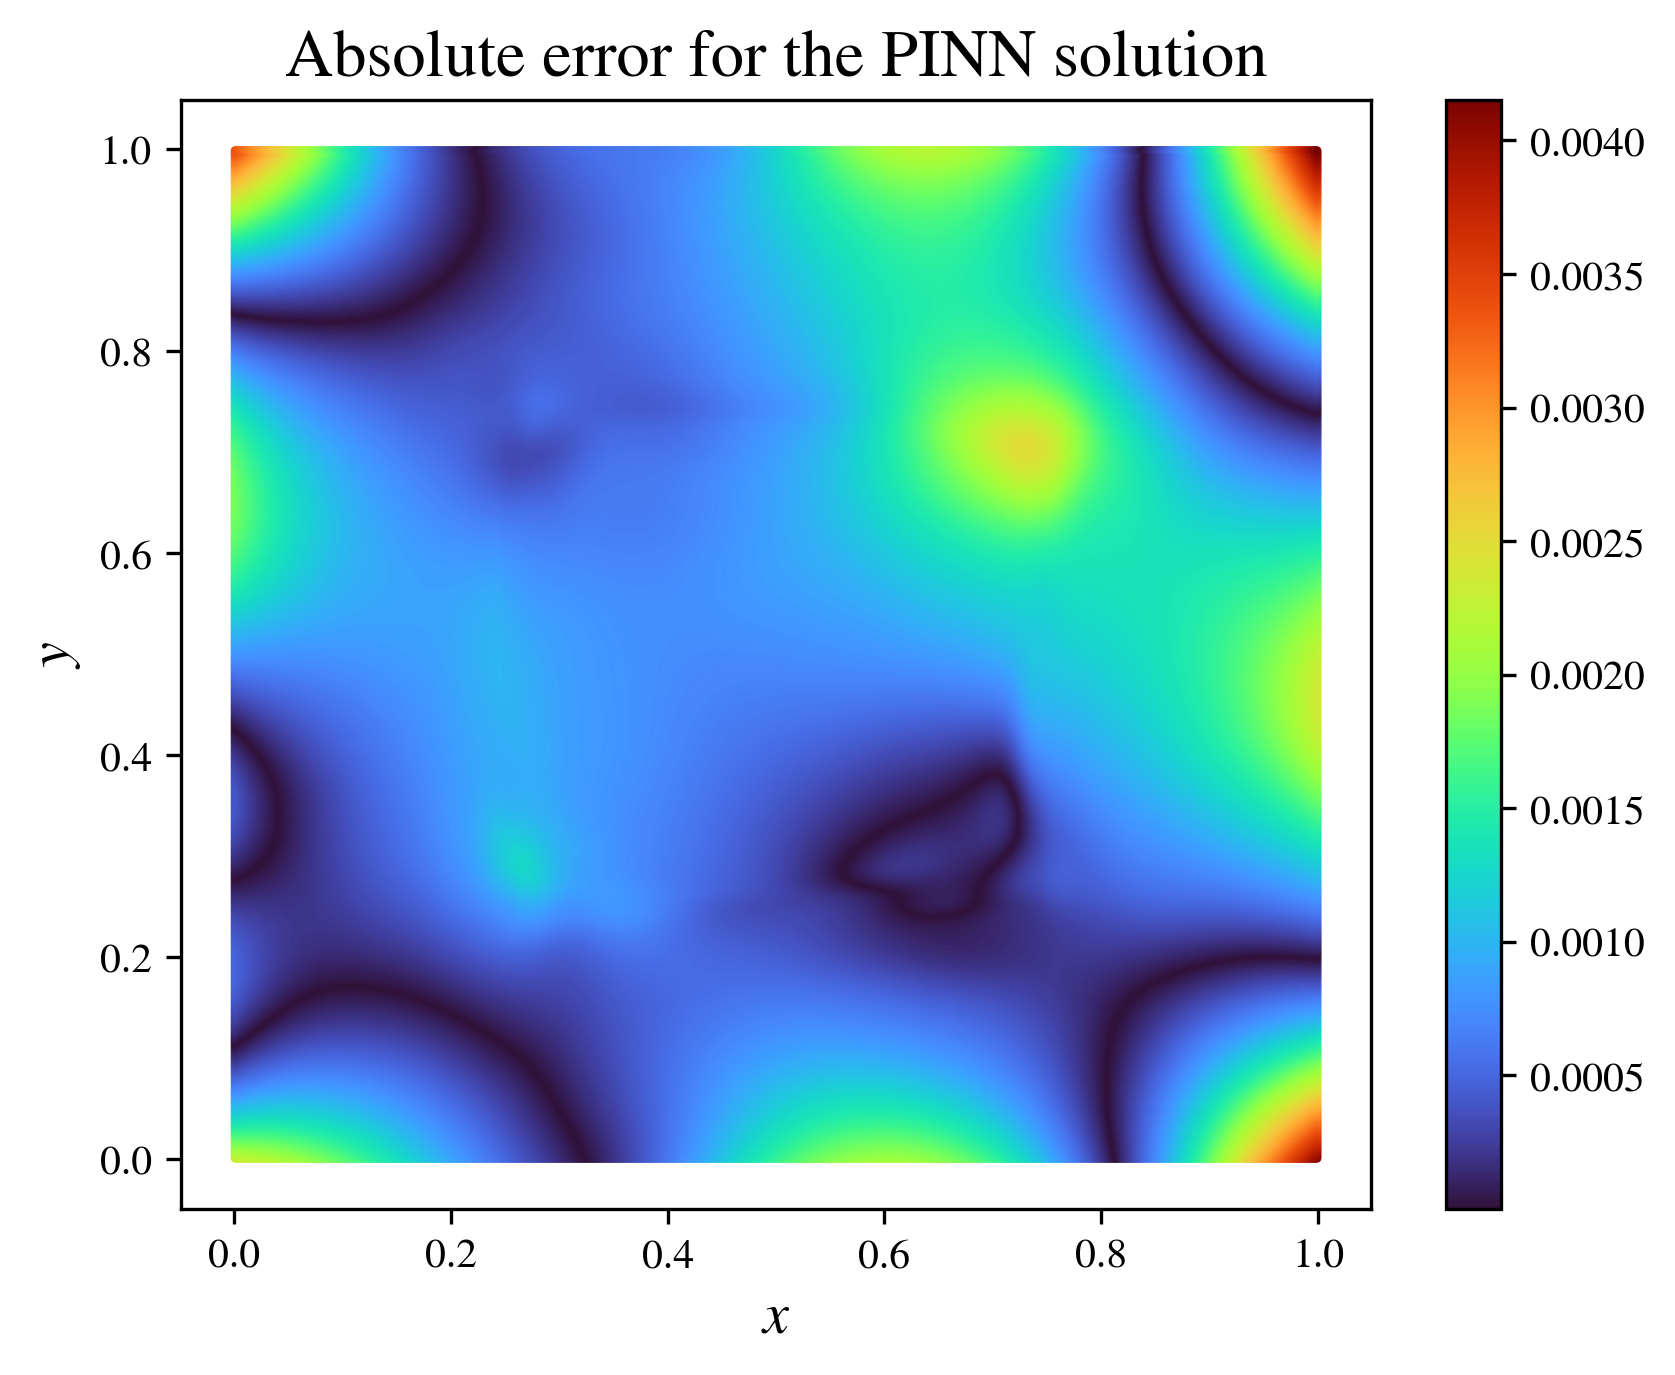
\includegraphics[width=0.7\linewidth]{Project1XPINNs/figures/Poisson/discrete_single_Poisson_error.pdf.png}
    \caption{PINN absolute error with discontinuous residual.}
    \label{fig:pinn_disc_error}
\end{figure}

\begin{figure}[h]
    \centering
    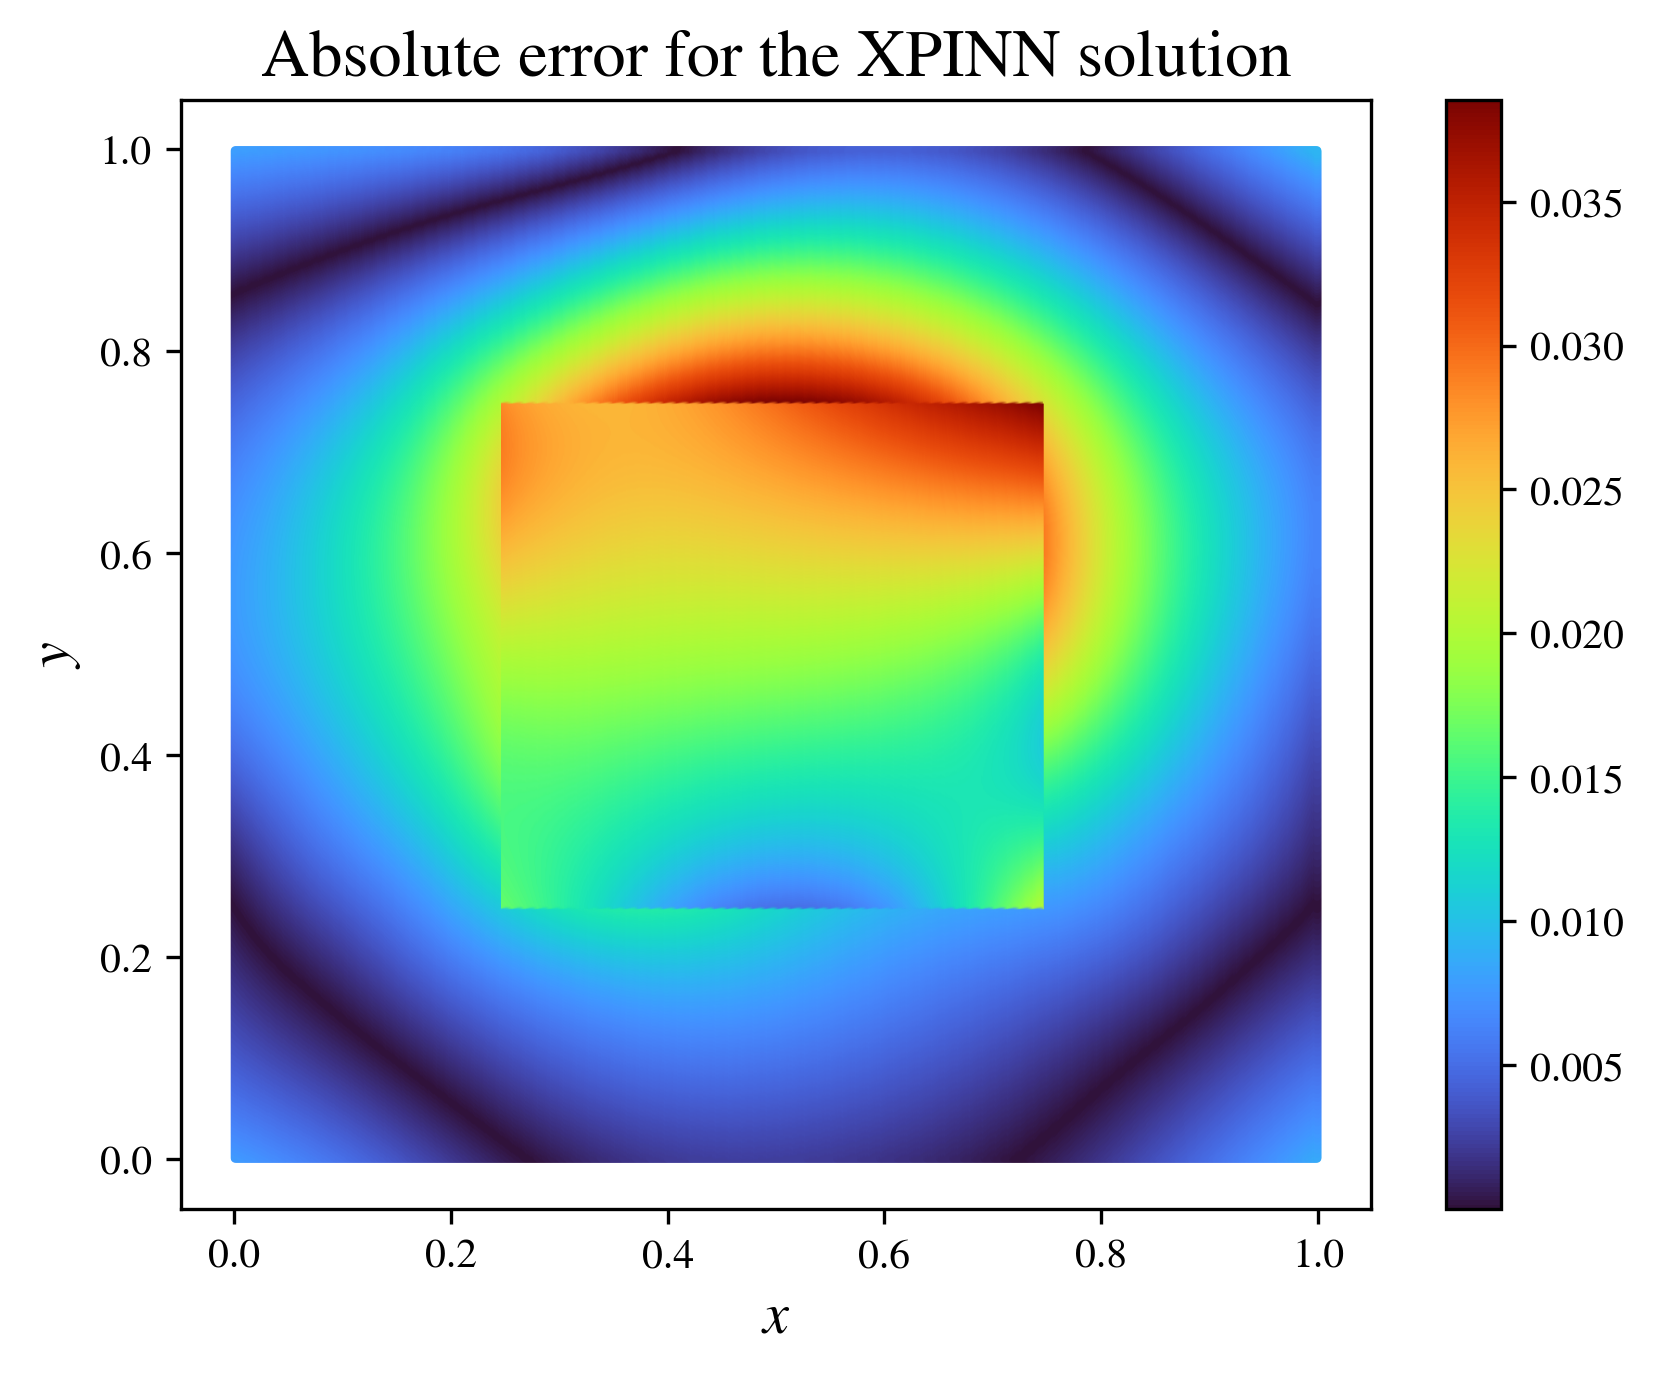
\includegraphics[width=0.7\linewidth]{Project1XPINNs/figures/Poisson/discrete_xpinn_Poisson_error.png}
    \caption{XPINN absolute error with discontinuous residual.}
    \label{fig:xpinn_disc_error}
\end{figure}


\subsection{Navier-Stokes Equation}
\subsubsection{Problem Formulation}
Finally, we consider the Navier Stokes problem as described in the FEATFLOW benchmark suite \cite{DFG}. This problem is a simulation of an incompressible 2D fluid flow hitting a cylinder in a rectangle. In the DFG benchmark 2D-1, the PDE conditions are given by
\begin{equation}
    -\nu \nabla^2 \mathbf{u} + (\mathbf{u} \cdot \nabla)\mathbf{u} + \nabla p = \mathbf{0}, \quad \nabla \cdot \mathbf{u} = 0,
\end{equation}
where $\nu = 0.001$. In our notation, we will isolate the $x$- and $y$-flow as $u$ and $v$ respectively. From this, we can express the PDEs for the second-order spatial derivatives, as well as the equation for zero convergence due to incompressibility as
\begin{equation}
\begin{cases}
-\nu(u_{xx} + u_{yy})+uu_x+vu_y+p_x = 0, \\
-\nu(v_{xx} + v_{yy})+uv_x+vv_y+p_y = 0, \\
u_x + v_y = 0.
\end{cases}
\end{equation}

In order to impose the zero divergence condition, we let our network $\mathcal{N}_\theta$ predict both the stream function $\psi$ and the pressure $p$, with
\begin{equation}
    \mathcal{N}_\theta : \mathbb{R}^3 \to \mathbb{R}^2, \quad (x,y,t)\to (\psi, p).
\end{equation}
We obtain $u$ and $v$ from the equations $u=\psi_y$ and $v=-\psi_x$.

This problem includes three different boundary conditions.
First, we have the boundary for the upper and lower walls, as well as around the edge of the cylinder.
On these walls, we require the flow to be exactly zero.
In the DFG benchmark 2D-1 \cite{DFG}, the lower and upper walls are notated as $\Gamma_1 = [0,2.2]\times 0$ and $\Gamma_3 = [0,2.2]\times 0.41$ respectively, and the boundary as $S=\partial B_r(0.2,0.2)$.
The no-slip boundary condition is defined as
\begin{align*}
    u_{|\Gamma_1} = u_{|\Gamma_3} = u_{|S} &= 0, \\
    v_{|\Gamma_1} = v_{|\Gamma_3} = v_{|S} &= 0.
\end{align*}
On the left boundary we enforce polynomial inflow.
The left boundary is $\Gamma_2 = 0\times [0,0.41]$ and the polynomial inflow is given by
\begin{equation*}
    u=\frac{4Uy(0.41-y)}{0.41^2}, \quad v=0
\end{equation*}
where $U=0.3$.
Finally, on the right boundary we have the do-nothing boundary condition.
The boundary is $\Gamma_4=2.2\times[0,0.41]$, and the condition is given by
\begin{equation*}
    \nu u_x - p = 0, \quad \nu u_y = 0.
\end{equation*}

\subsubsection{Results}